\documentclass{jhps}
\usepackage{silence}
\WarningFilter{todonotes}{The length}
\WarningFilter{caption}{Unsupported}
\WarningFilter{caption}{Forced redefinition}
\WarningFilter{caption}{The option}
\WarningFilter{caption}{Unknown document}
%\WarningFilter{hyperref}{Suppressing}

\usepackage{array}
\usepackage{cite}
\usepackage{amsmath,amssymb,amsfonts}
\usepackage{algorithmic}
\newsavebox{\imagebox}
\usepackage{textcomp}
\usepackage{lstautogobble}
\usepackage[listings,skins,breakable,raster,most]{tcolorbox}
\usepackage{numprint}
\usepackage{adjustbox}
\usepackage{tikz}
\usetikzlibrary{positioning,shapes,arrows,fit,backgrounds}
\usepackage{booktabs}
\usepackage{multirow}
\usepackage{tabularx}
\usepackage{mathtools}
\usepackage{newfloat}
\usepackage{subcaption}
\usepackage{placeins}
\usepackage{etoolbox}

% TICKS hack
\makeatletter \global\let\tikz@ensure@dollar@catcode=\relax \makeatother

\AtBeginEnvironment{tabular}{\scriptsize}
\AtBeginEnvironment{tabularx}{\scriptsize}

\crefname{codecount}{Code}{Codes}

\DeclareFloatingEnvironment[fileext=frm,placement={!ht},name=Listing,within=section]{listing}
%\DeclareFloatingEnvironment[fileext=xyz,placement={!ht},name=Cluster\,Overview,within=section]{figure}


\usepackage{verbatimbox}
\usepackage{todonotes}
\newcommand{\jk}[1]{\todo[inline]{JK:\@#1}}
\newcommand{\eb}[1]{\todo[inline, color=GreenYellow]{EB:\@#1}}

%\definecolor{tblhead}{rgb}{0.63, 0.79, 0.95}
%\newcolumntype{$}{>{\global\let\currentrowstyle\relax}}
%\newcolumntype{^}{>{\currentrowstyle}}
%\newcommand{\rowstyle}[1]{\gdef\currentrowstyle{#1}%
%    #1\ignorespaces
%  }

%\crefname{figure}{Cluster\,Overview}{Cluster\,Overviews}
%\crefname{subcluster}{Sub-Cluster\,Overview}{Sub-Cluster\,Overviews}
\crefname{sublisting}{Listing}{Listings}
%\setcounter{figure}{0}
%\setcounter{subcluster}{0}

\lstset{%
	autogobble=true,
}

\begin{document}

\JHPSissue{0}   % keep 0 until the issue is assigned
\JHPSkeywords{Holistic log data analysis, K computer, FEFS, Tofu, MPI-IO}

  % Author macro takes Name, Institution, Optional Link to the person, Optional Email
\JHPSauthor{Yuichi Tsujita}{RIKEN Center for Computational Science, Kobe, Japan}{}{yuichi.tsujita@riken.jp}
\JHPSauthor{Yoshitaka Furutani}{Fujitsu Limited, Tokyo, Japan}{}{}
\JHPSauthor{Hajime Hida}{Fujitsu Limited, Tokyo, Japan}{}{}
\JHPSauthor{Keiji Yamamoto}{RIKEN Center for Computational Science, Kobe, Japan}{}{}
\JHPSauthor{Atsuya Uno}{RIKEN Center for Computational Science, Kobe, Japan}{}{}


\title{Holistic I/O Activity Characterization Through Log Data Analysis of Parallel File Systems and Interconnects}

% add the section numbers to the listings/figures/tables
\counterwithin{lstlisting}{section}
\counterwithin{figure}{section}
\counterwithin{table}{section}

\maketitle

\begin{abstract}
The performance of HPC systems is increasing with a rapid growth in the number of
compute nodes and CPU cores.
Meanwhile, I/O performance is one of the bottlenecks in improving HPC system performance.
Recent HPC systems utilize parallel file systems such as GPFS and Lustre
to cope with the huge demand of data-intensive applications.
Although most of the HPC systems provide performance tuning tools on compute nodes,
there is not enough chance to tune I/O activities on parallel file systems,
including high speed interconnects among compute nodes and file systems.
We propose an I/O performance optimization framework that uses log data of
parallel file systems and interconnects in a holistic way
for improving performance of HPC systems including I/O nodes and parallel file systems.
We demonstrate our framework at the K computer with two I/O benchmarks
for the original and the enhanced MPI-IO implementation.
The analysis by the framework reveals the effective utilization of parallel file systems
and interconnects among I/O nodes in the enhanced MPI-IO implementation.
\end{abstract}


\section{Introduction}

HPC systems have been facing the performance gap between computing power and I/O performance.
Parallel file systems such as GPFS~\cite{gpfs:usenix02} and Lustre~\cite{lustre:web} provide
a large amount of storage capacity with high I/O bandwidth to bridge the gap.
Most of the I/O optimization research efforts have addressed to improve I/O performance
of their implementations in an empirical way using I/O benchmarks rather than
analyzing I/O activities on target parallel file systems and data transfers through interconnects.
With an increase in the number of compute nodes and target I/O nodes,
it is quite difficult to tune an implementation only through such benchmark runs.

A profiling tool named Tofu PA~\cite{profiler:fujitsu-tech-si} is provided on the K computer,
which acquired statistical information called Tofu PA information regarding communication
in the Tofu interconnects~\cite{tofu:micro2012} on used compute nodes, with the purpose
to tune communications among compute nodes.
However, there were no tools to get the Tofu PA information of Tofu interconnects
among I/O nodes and I/O activities of its parallel file systems.
A well-balanced I/O workload among compute nodes, I/O nodes, and parallel file systems
is required to optimize I/O operations. Without knowing the status of I/O nodes
and parallel file systems, it is quite difficult to tune I/O operations in HPC applications.

It is expected that the utilization of statistics log data of file system servers and
interconnects provides quite useful metrics for I/O performance tuning by examining statistics
of I/O request operations or data packet transfers through interconnects.
In this context, we have proposed a framework that monitors data transfers
on Tofu interconnects on I/O nodes and I/O activities of parallel file systems
with the help of log data collected in the system administration
in our workshop paper~\cite{tsujita:hpc_iodc20}.
To our best knowledge, this is the first work to utilize data transfer information of
Tofu interconnects on I/O nodes among the HPC systems using Tofu interconnects
in tuning I/O operations.
The framework consists of several components: log data collected by
{\itshape fluentd}~\cite{fluentd:web}, a PostgreSQL database that keeps a large amount
of executed job information (JOB-DB),
compute-node information table, and analysis function.

Given a unique ID for each job (JOB-ID), the analysis function of the framework
provides us data such as averaged values of essential I/O activities on used OSSes,
bandwidth utilization of Tofu interconnects on I/O nodes, and heat-maps about
I/O performance of used OSTs from the log data with the help of the JOB-DB.
In this paper, we show how such analyzed data can be used for further performance improvements
by examining I/O bottlenecks or unbalanced situations in I/O workload among I/O nodes.

Compared with our previous paper~\cite{tsujita:hpc_iodc20},
we have made further analysis by having additional
optimizations in an enhanced MPI-IO with and without two-phase I/O
in order to show its usefulness
in investigating performance advantages achieved by
the enhanced MPI-IO compared with the original MPI-IO
through two I/O benchmark runs.
We have found new explicit differences in metrics which are given by the framework
in not only write operations but also read operations.

Rest of this paper is organized as follows.
In Sec.~\ref{sec:RELATED_WORK}, we discuss the related work.
A system overview including a file I/O subsystem of the K computer,
which is an evaluated platform for the proposed framework,
is explained in Sec.~\ref{sec:K_COMP}.
In Sec.~\ref{sec:ANAL_SYS}, we present the proposed analysis framework.
We also explain an enhanced MPI-IO implementation at the K computer
in Sec.~\ref{sec:EARTH}, where we briefly present its advanced functions
relative to the original MPI-IO.
In Sec.\ref{sec:EVAL}, we demonstrate experimental evaluations
for the proposed framework at the K computer, and we discuss the usefulness
of the proposed framework through examinations about performance improvements
achieved by the enhanced MPI-IO.
Finally we conclude the paper in Sec.~\ref{sec:CONCLUSIONS}.

\section{Related Work}
\label{sec:RELATED_WORK}

I/O bottlenecks in various applications were studied in \cite{xie:sc12,saini:hipc12}.
These studies showed various characteristics in terms of I/O access patterns performed
by applications on HPC systems using Lustre file systems.
I/O monitoring at storage system level has been studied
in \cite{isc14:kunkel,uselton:cug13,madireddy:nas17}.
Multi-platform study using system logs of file systems has been reported
in \cite{luu:HPDC2015}.

Log data collection and analysis for performance tuning have been done in
server-side analysis~\cite{liu:fast2014,liu:sc16,xu:cug16}.
Detailed study in production runs has been done in \cite{patel:sc19}
by analyzing server-side log data.
Even sufficient logging of each server-side component did not provide causal relationships
between client and server-side activities.

Interconnects are also one of the key components in HPC systems. Monitoring data transfers of
interconnects has provided a hot-spot of traffic congestion for instance,
and such approaches have succeeded in analysis of application activities associated with
the traffic condition~\cite{zimmer:cug16,kumar:DSN2018}.
However, it is not sufficient to characterize I/O activities on parallel file systems
in HPC systems.

Recently, holistic I/O monitoring has been proposed
in several research works~\cite{lockwood:cug18,yang:nsdi2019}.
Lockwood et al. have proposed a holistic I/O monitoring framework
named TOKIO~\cite{lockwood:cug18}.
It consisted of several components for monitoring, analysis and visualization
for administrators and users. The work in \cite{yang:nsdi2019} has proposed
a monitoring framework named Beacon.
This framework provides a collection of monitoring tools for Metadata Servers (MDSes)
and Object Storage Servers (OSSes) and analysis functions,
including some visualization interface. These works are similar to our work regarding
holistic approach in characterization of I/O activities.

In contrast, our work addresses analysis of I/O activities through holistic log data analysis
of Tofu interconnects and parallel file systems including associated I/O nodes.
The uniqueness of this work is a holistic analysis framework using data transfer status
on interconnects among I/O nodes and associated I/O activity traces at parallel file systems.


\section{K computer and Its File System Monitoring}\label{sec:K_OVERVIEW}
\label{sec:K_COMP}

\subsection{Overview of the K computer}

The K computer finished its operation for about seven years in August 2019.
The system had two-layered file systems, a local file system (LFS)
and eight volumes of a global file system (GFS) as shown in Fig.~\ref{fig:K_OVERVIEW}.
%
\begin{figure}[tb]
\centering
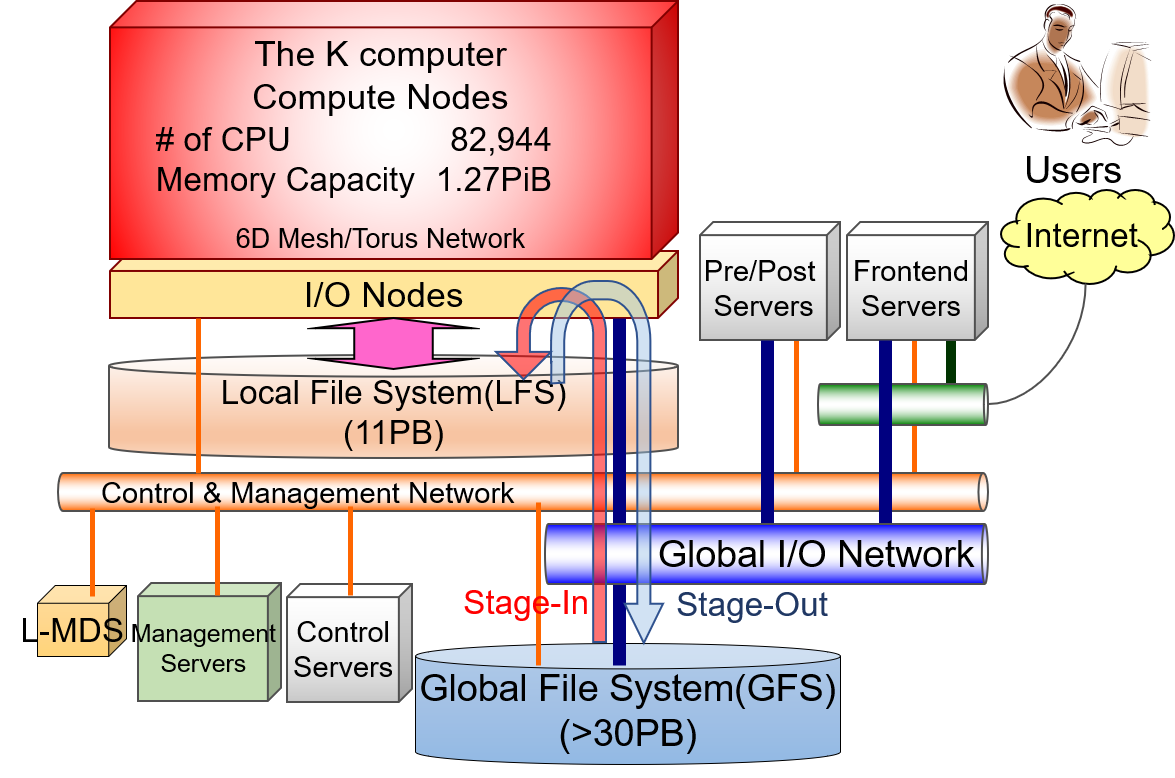
\includegraphics[width=0.6\textwidth]{K-system-overview.png}
\caption{System configuration of the K computer}
\label{fig:K_OVERVIEW}
\end{figure}
%
The LFS was a scratch high-performance storage space which was used during computations,
while the GFS was used to store programs and data with high redundancy.
An enhanced Lustre named FEFS (Fujitsu Exabyte File System)~\cite{fefs:fujitsu-tech-si}
developed by Fujitsu was used to build both file systems,
where the FEFS was based on Lustre version 1.8 at the K computer.
The K computer consisted of 82,944 compute nodes and 5,184 I/O nodes,
where every system rack consisted of 96 compute nodes and six I/O nodes.
Every compute node and I/O node were connected through the Tofu interconnect
in 6D mesh/torus network represented by X, Y, Z, A, B, and C.
Tofu links of X, Z and B were connected in torus configuration,
while those of Y, A, and C were in mesh configuration.
However, torus configuration of the Z-link was available only in I/O accesses
because I/O nodes were included in only I/O accesses.
In other cases, the Z-link was used in mesh configuration for inter-node communications
by application jobs.

Figure~\ref{fig:SUBSET_SYSRACK_K} depicts the configuration of a subset of system racks
and I/O accesses from compute nodes towards the LFS.
%
\begin{figure}[tb]
\centering
%% \includegraphics[width=0.7\textwidth]{K-system-rack-config.png}
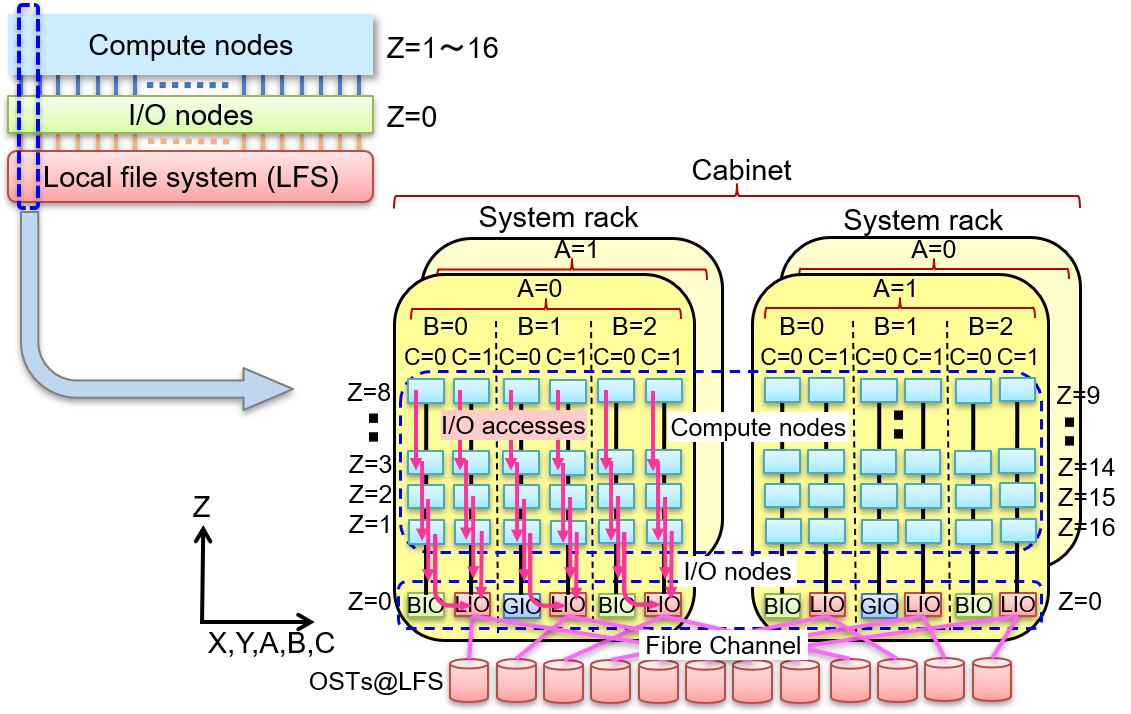
\includegraphics[width=0.8\textwidth]{K-system-rack-config-mod.png}
\caption{Subset of system racks of the K computer and I/O accesses from compute nodes
towards the LFS}
\label{fig:SUBSET_SYSRACK_K}
\end{figure}
%
Each cabinet consists of two system racks, which have two groups separated
by the A-link position (A=0 and 1) consisting of 48 compute nodes each.
Every compute node was located on Z-link positions ranging from 1 to 8 and
from 9 to 16 in the groups of A=0 and 1, respectively, while I/O nodes were
on Z=0 in the both groups.
Boot-I/O nodes (BIOs) were responsible for system software start-up and
Global I/O nodes (GIOs) were the gateways in accessing the GFS.
The LFS is accessible from compute nodes through OSSes running on the local-I/O nodes (LIOs).
Every node including I/O nodes consisted of Tofu network router (TNR)~\cite{tofu:micro2012}
where each TNR had 10 communication links (X+, X-, Y+, Y-, Z+, Z-, A, B+, B-, and C)
to construct the 6D mesh/torus network.

The number of available OSTs at the LFS is uniquely configured based on the shape of
assigned compute nodes according to the I/O zoning scheme~\cite{sumimoto:LUG2011}.
I/O zoning scheme has been introduced in order to mitigate I/O interference on OSTs
and I/O nodes among jobs by assigning I/O nodes and OSTs on the same Z-link
with used compute nodes.
We illustrate I/O accesses from compute nodes
at the system rack in the left side in Fig.~\ref{fig:SUBSET_SYSRACK_K}.
I/O nodes on the same Z-links are configured to work with compute nodes which
issue I/O requests, and those I/O nodes
take part in data transfers during I/O accesses on the LFS.
It is noted that an I/O path from each compute node is automatically routed to
an I/O node (either of BIO, GIO, and LIO) on the same Z-link,
then routed to a target OSS running on an LIO.

Performance profiling tools including Tofu PA addressed to tune performance of compute nodes
and communications among compute nodes.
It is noted that the similar tools are available at Fugaku
as remarked in FAQ of \cite{fugaku_info:web}.
The tools have succeeded to leverage computing potential of the K computer,
especially in tuning applications utilizing a large number of compute nodes.
The only way to tune I/O operations is benchmark evaluations
because there was not any I/O profiling tool for users to profile activities
of I/O nodes and parallel file systems including the Tofu PA information among I/O nodes.
Therefore, it was quite difficult to tune I/O operations using only the existing profiling tools.

\subsection{Log collection for monitoring the LFS}

In the K computer operation, we have collected log data from servers associated with the LFS as shown in Figure~\ref{fig:Log-collect-K}.
%
\begin{figure}[tb]
\centering
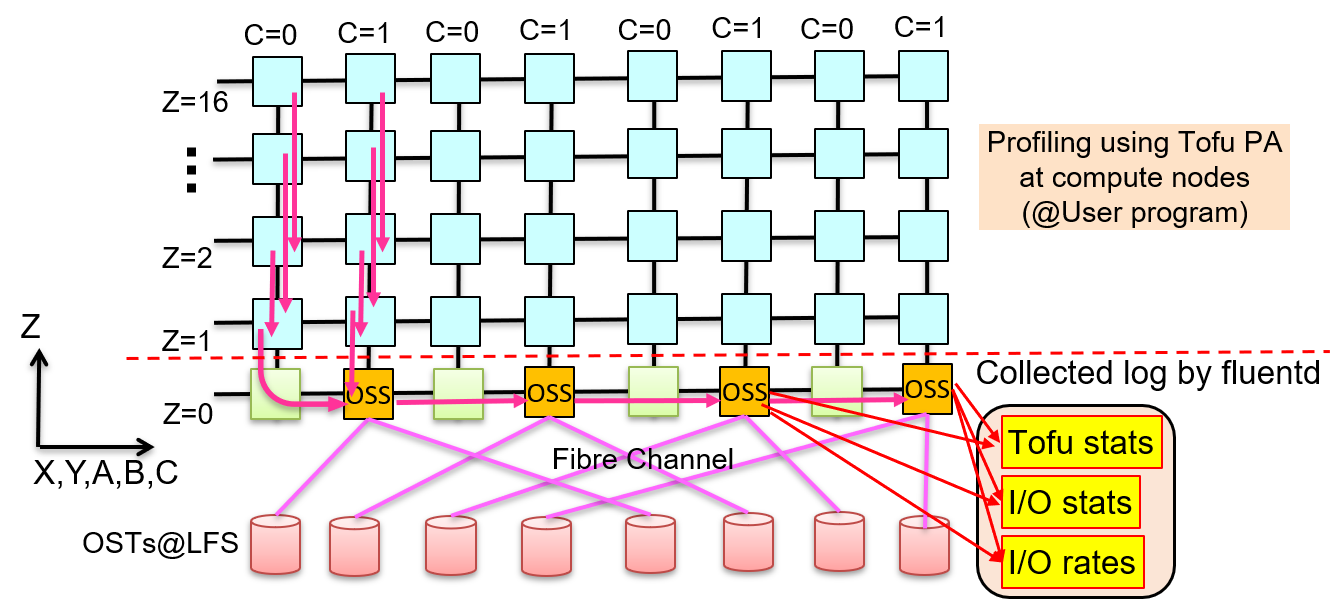
\includegraphics[width=0.72\textwidth]{Log-collect-K-ext.png}
\caption{Log collection from I/O nodes}
\label{fig:Log-collect-K}
\end{figure}
%
We have deployed {\itshape fluentd} to collect performance metrics associated with
I/O operations from 5,184 I/O nodes including 2,592 LIOs which also acted as OSSes for the LFS.

% The number of available OSTs at the LFS is uniquely configured based on the shape of
% assigned compute nodes according to the I/O zoning scheme~\cite{sumimoto:LUG2011}.
% I/O zoning scheme has been introduced in order to mitigate I/O interference on OSTs
% and I/O nodes among jobs by assigning I/O nodes and OSTs on the same Z-link
% with used compute nodes.
% All assigned I/O nodes for each job take part in data transfers during I/O accesses on the LFS.
% It is noted that an I/O path from each compute node is automatically routed to an I/O node
% on the same Z-link, then routed to a target OSS on an LIO.

The proposed analysis framework utilizes the following log data from a large amount of collected information by {\itshape fluentd}.
%
\begin{itemize}
\item {\tt Tofu stats}: Data transfer status metrics of I/O nodes on each Tofu interconnect link
(the number of transferred packets, amount of transferred data size, and others)
\item {\tt I/O stats}: Statistics of I/O requests obtained from
{\tt /proc/fs/lustre/ost/OSS/ost io/stats} on every OSS
\item {\tt I/O rates}: Amount of size in read and write operations on every OST
\end{itemize}
%
Only the {\tt I/O stats} have been collected at 1 minute intervals, while the remainings have been
collected at 10 minute intervals.
The 10 minute intervals were selected for the I/O related monitoring as trial
in a conservative manner not to affect I/O node activities for stable production runs
from our empirical study in the last few months of the K computer operation.
Limited storage space for the I/O related log-collection is another reason
in the last few months of the K computer operation since we have already collected
a huge size of recorded information on the log-collection server
from other high-priority components of the K computer for a long time.

The {\tt Tofu stats} consist of the following packet processing metrics of the 10 links,
which are obtained from a TNR of each I/O node through the Tofu PA information
in each 10 minutes interval:
%
\begin{itemize}
\item Cycle counts until target transfer buffer was available in packet transfers
\item Amount of transferred data size
\end{itemize}
%
It is noted that the cycle counts in the Tofu stats correspond to congestion status
since unavailability of transfer buffers in packet processing closely corresponds to
packet transfer congestion.
We enforced to retrieve those metrics from a TNR at every I/O node
during the K computer operation for about a few months
until the end of the K computer operation.

The {\tt I/O stats} consist of the same statistics with those of a standard Lustre,
where we especially focus on the three statistics; {\tt req\_qdepth}, {\tt req\_active},
and {\tt req\_waittime}.
Such statistics give the status of I/O requests coming from compute nodes through I/O nodes.
For instance, a large value in both {\tt req\_qdepth} and {\tt req\_waittime} indicates
very busy status of OSSes or idle status of OSSes waiting for the next operation
due to heavy load of an MDS before I/O accesses for instance.
Such a situation is not suitable for effective I/O operations.
{\tt req\_active} indicates the number of active threads for I/O operations.
High numbers in only {\tt req\_active} indicate a very good condition in terms of I/O accesses.
The {\tt I/O rates} give us I/O throughput status at each OST over time.
Collected I/O throughput information is expected to show I/O behavior that happened
on each OST.
Due to the reasons described above, we have examined I/O activities
in the two I/O benchmark runs at 10 minute intervals as trial,
where each I/O benchmark run took around 10 minutes so that we could observe
I/O activities of each I/O benchmark run.
Minimization of monitoring interval time is our future work in our next HPC system.

\subsection{Database for executed jobs}

The PostgreSQL database server has collected information of executed jobs at the K computer
on the JOB-DB database.
The JOB-DB keeps used compute nodes, elapsed time, and start and finish times of job execution,
for instance by associating with a JOB-ID.
Therefore, we can refer to information about a target job from the JOB-DB by specifying a JOB-ID.

\section{Analysis Framework for I/O Activities}
\label{sec:ANAL_SYS}

Figure~\ref{fig:LOG_ANAL_SYS} depicts an overview of the implemented analysis framework,
which is connected with associated log data collected by {\itshape fluentd}
and the JOB-DB to analyze I/O activities on I/O nodes and the LFS.
%
\begin{figure}[tb]
\centering
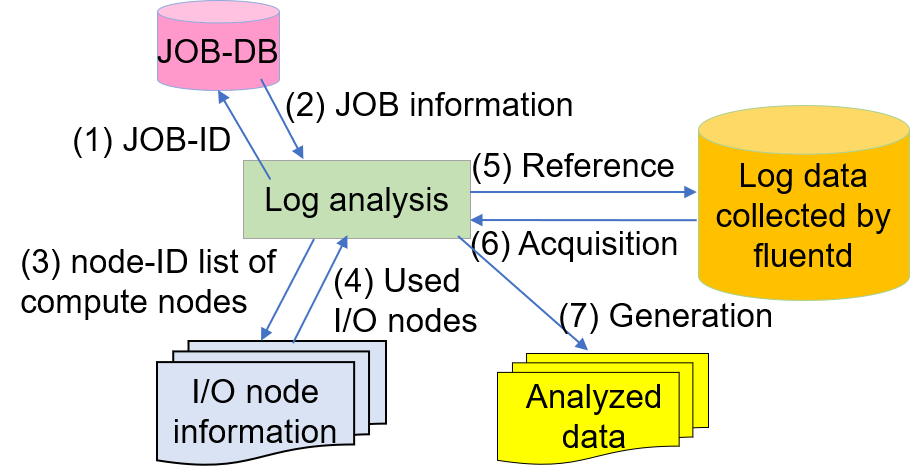
\includegraphics[width=0.6\textwidth]{Log-anal-system.png}
\caption{Functional overview of implemented analysis framework}
\label{fig:LOG_ANAL_SYS}
\end{figure}
%
Given a target JOB-ID, the framework retrieves information of the JOB-ID
such as 6D mesh/torus network positions of used compute nodes and names of
used system racks.
Such information about used compute nodes and system racks is utilized
to find used I/O nodes including LIOs from the I/O node table
because the assigned I/O node layout is configured by the shape of assigned compute nodes.
Besides, start and finish times of the target job obtained from the JOB-DB were
used to pick up essential information associated with the JOB-ID
from a large amount of log data collected by {\itshape fluentd}.

Once the framework collects all essential information, its log analysis function
figures out and gives the following information for the given JOB-ID:
\begin{itemize}
\item Maximum waiting time of each interconnect at each used I/O node
\item Bandwidth utilization ratio of the interconnects relative to the theoretical bandwidth
\item I/O performance in both write and read operations on each used OST
\end{itemize}
%

The former two performance values are calculated by using the packet transfer metrics
obtained from the TNR. The function converts the cycle counts into time values
in the unit of second for the maximum waiting times.
While the bandwidth utilization ratio during the job running is obtained by
dividing the peak bandwidth of the job by the theoretical bandwidth,
where the peak bandwidth is obtained from throughput values collected
in an elapsed time of the specified job. In the proposed framework,
we use the maximum bandwidth utilization to examine effectiveness
in packet transfer associated with I/O operations.

While the I/O performance values were obtained by dividing an amount of data size
in read and write operations by a monitoring
interval time (600 seconds in the current configuration) in order to know
I/O throughput at each used OST.
Once the analysis function is executed, data are stored in the CSV format
and associated heat-map image data are stored in the PNG format.

\section{Enhanced MPI-IO Implementation: EARTH on K}
\label{sec:EARTH}

MPI-IO is an I/O interface including parallel I/O in the MPI standard~\cite{mpi-forum:web}.
An MPI library for the K computer supports MPI-IO functions for the FEFS
using ROMIO~\cite{thakur:romio}.
Although two-phase I/O optimization of ROMIO improves collective MPI-IO performance,
the implementation on the K computer uses an old implementation of ROMIO
which is not optimized for Lustre.
Therefore, the original MPI-IO implementation is not suitable
for the FEFS to achieve high I/O performance.

The recent ROMIO with the improved two-phase I/O for Lustre has a potential
to improve performance on the FEFS.
An enhanced implementation named "EARTH on K"
(hereinafter, EARTH)~\cite{tsujita:WS_EuroMPI2014,tsujita:hpcasia18}
has been developed for the K computer by introducing
the improved two-phase I/O with some performance optimizations
for collective MPI-IO at the FEFS.

Its advanced functions are summarized in the following three key optimization parameters
described by {\tt agg}, {\tt req}, and {\tt rr}, respectively:
%
\begin{itemize}
\item {\tt agg}: Striping-aware aggregator layout
\item {\tt req}: I/O throttling and associated stepwise data aggregation
with a given number of I/O requests per step
\item {\tt rr}: Round-robin aggregator layout among compute nodes
\end{itemize}
%

The striping-aware aggregator layout mitigates data transfer congestion
by suitable layout of processes performing I/O (aggregators)
in collective MPI-IO operations using ROMIO.
Figure~\ref{fig:AGG_STR_AWARE} shows aggregator layouts with and
without striping awareness in accessing four OSTs by 16 aggregators,
where numbers in circles represent MPI ranks
and the numbers ranging from "{\tt i}" to "{\tt iv}" represent
the order of striping accesses.
%
\begin{figure}[htb]
\centering
\begin{minipage}[t]{0.42\textwidth}
\centering
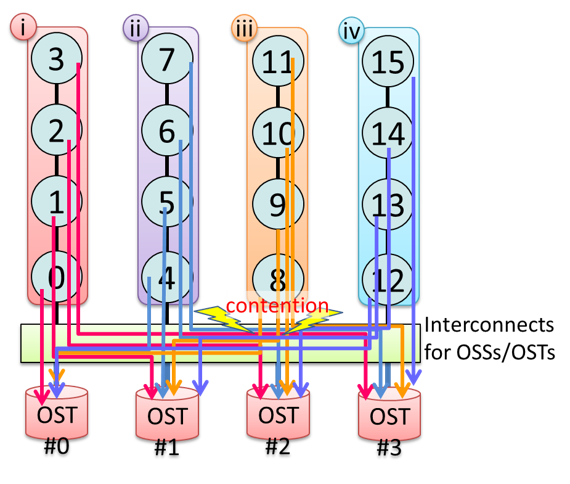
\includegraphics[width=0.96\textwidth]{MPI-IO-non-agg-opt.png}
\subcaption{Without striping-awareness}
\label{fig:WO_STR_AWARE}
\end{minipage}
\noindent
\begin{minipage}[t]{0.42\textwidth}
\centering
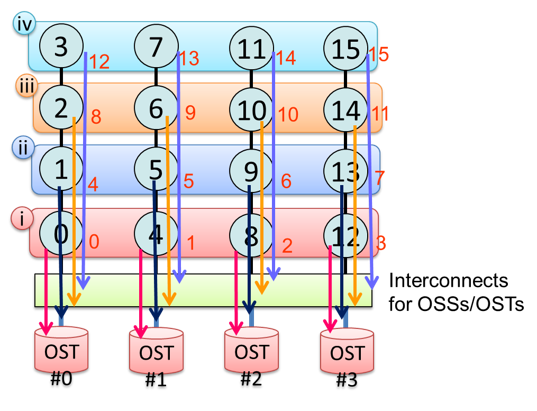
\includegraphics[width=0.96\textwidth]{MPI-IO-with-agg-opt.png}
\subcaption{With striping-awareness}
\label{fig:WITH_STR_AWARE}
\end{minipage}
\caption{Aggregator layouts with and without striping awareness}
\label{fig:AGG_STR_AWARE}
\end{figure}
%
By placing aggregators in the order of MPI ranks
as shown in Fig.~\ref{fig:AGG_STR_AWARE}\subref{fig:WO_STR_AWARE},
we may face contention in a path towards target OSTs.
On the other hand, a striping-aware layout shown in
Fig.~\ref{fig:AGG_STR_AWARE} \subref{fig:WITH_STR_AWARE},
renumbering the order of aggregators in the red-colored numbers,
eliminates data transfer congestion on every I/O path
because I/O flows of every I/O path towards a target OST are
evenly distributed for a striping access pattern against OSTs.

Figure~\ref{fig:IO_THROT} depicts an overview of I/O throttling
scheme done by 192 aggregators towards 12 OSTs.
%
\begin{figure}[htb]
\centering
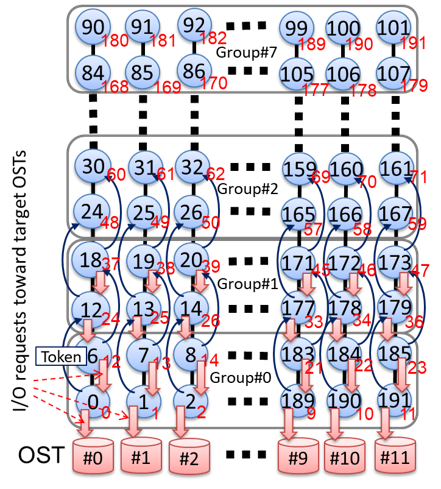
\includegraphics[width=0.42\textwidth]{MPI-IO-throttling.png}
\caption{I/O request throttling with stepwise data aggregation}
\label{fig:IO_THROT}
\end{figure}
%
Numbers in circles represent MPI ranks, and red-colored numbers neighboring
to the circles are the aggregator layout orders.
We may have I/O request contention on OSTs
if we have I/O requests simultaneously from all aggregators.
The I/O throttling shown in this figure alleviates I/O request contention
on OSTs by issuing I/O requests from aggregators in a stepwise manner
as divided into multiple groups.
The number of groups can be tuned by the program.
Stepwise data aggregation is an optimization associated
with the I/O throttling, where congestion of data transfer
among compute nodes can be mitigated.

Figure~\ref{fig:AGG_RR_LAYOUT} illustrates blocked and round-robin
aggregator layouts, where we have eight aggregators from 16 processes
deployed among four compute nodes in a blocked layout.
%
\begin{figure}[htb]
\centering
\begin{minipage}[t]{0.36\textwidth}
\centering
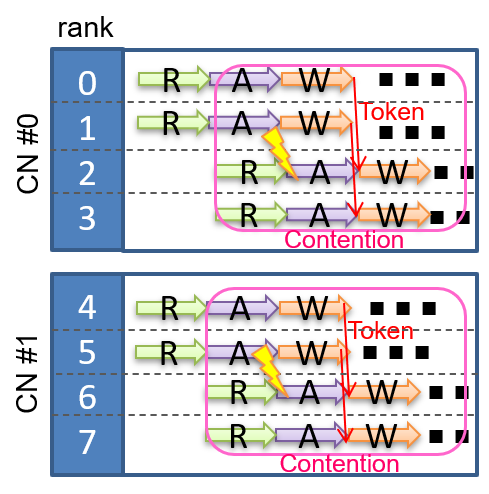
\includegraphics[width=0.96\textwidth]{MPI-IO-agg-block_layout.png}
\subcaption{Blocked layout}
\label{fig:BLK_LAYOUT}
\end{minipage}
\noindent
\begin{minipage}[t]{0.36\textwidth}
\centering
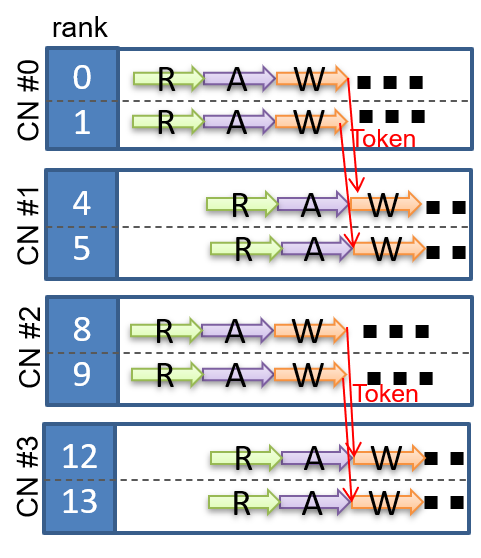
\includegraphics[width=0.96\textwidth]{MPI-IO-agg-rr_layout.png}
\subcaption{Round-robin layout}
\label{fig:RR_LAYOUT}
\end{minipage}
\caption{Aggregator layouts with blocked and round-robin manners with
I/O throttling and step-wise data aggregation in write operations}
\label{fig:AGG_RR_LAYOUT}
\end{figure}
%
Horizontal arrows remarked by "R", "A", and "W" represent
read, data aggregation, and write phases in collective write
operations using two-phase I/O, respectively.
I/O throttling scheme exchanges tokens among aggregators.
If we have a blocked aggregator layout as shown in
Fig.~\ref{fig:AGG_RR_LAYOUT}\subref{fig:BLK_LAYOUT},
every four processes in the two compute nodes ("CN \#0" and "CN \#1")
act as aggregators.
As a result, we may have contention inside the same compute node.
It is remarked that such layout leads to high I/O workload
in each node.
Meanwhile the round-robin aggregator layout in
Fig.~\ref{fig:AGG_RR_LAYOUT}\subref{fig:RR_LAYOUT}
can distribute I/O workload evenly
among compute nodes, and it also prevents aggregators
from I/O access congestion on the same compute node.
%% if we have multiple aggregators on a subset of compute nodes.

Although the above enhancements outperformed the original version
in an empirical study using I/O benchmark runs, there were not any examinations
to know performance impact of those optimizations because there were no tools
to characterize optimization effects in data transfers among I/O nodes and
I/O accesses against the LFS at the K computer.
By using the proposed framework, we examine their advanced features at the K computer
in the following section.

\section{Experimental Evaluation}
\label{sec:EVAL}

We evaluated the proposed framework at the K computer to compare
the original MPI-IO implementation and EARTH using IOR~\cite{IOR:web}
and HPIO~\cite{ching:ipdps06}.
For both benchmark runs, we initiated 12,288 processes on 3,072 compute nodes
forming a logical 3D layout of $8\times12\times32$ in order to eliminate I/O interference
from other jobs. According to the 3D layout of assigned compute nodes,
192 OSTs were assigned for parallel I/O, and we set 192 as a stripe count
to use all available OSTs.
We set 256~MiB and 64~MiB in stripe size in the IOR run and the HPIO run, respectively.

In both runs, 1,536 processes worked as aggregators, where aggregator assignment
was aligned to ascending order in MPI ranks from zero in the original MPI-IO,
while aggregator assignment was defined according to optimization configuration
of the EARTH.
In this paper, original stands for the original MPI-IO, while a combination of
the three optimization parameters ({\tt agg}, {\tt rr} and {\tt req}) indicates
the usage of EARTH.
Concerning the EARTH case, {\tt agg=1} stands for striping-aware aggregator layout
and {\tt rr=1} denotes round-robin aggregator layout among compute nodes.
A zero value in each case stands for deactivation in the corresponding layout optimization.
The last parameter req with a number describes the number of I/O requests
going to each OST per step in I/O throttling and stepwise data aggregation
except that {\tt req=0} denotes deactivation of I/O throttling and stepwise aggregation.

\subsection{Benchmark configuration}

We evaluated collective MPI-IO in both benchmark runs.
In both cases, we enabled two-phase I/O implemented in ROMIO.

\subsubsection{IOR}

The following command was executed in write operations to generate
a shared file of 3~TiB (= 256~MiB $\times$ 12,288) per iteration:
%
\begin{verbatim}
$ ior -i 5 -a MPIIO -c -U hints_info -k -m -vvv -w -t 256m -b 256m \
    -o ${TARGET_DIR}/test-IOR.dat -d 0.1
\end{verbatim}
%
The same command with just changing "-w" by "-r" was executed,
followed by write operations in every parameter configuration.
"{\tt hints\_info}", is a file describing some hints to set the number of processes per node,
and so forth.
A target file ({\tt test-IOR.dat}) was generated in the directory
({\tt \$\{TARGET\_DIR\}})
with 192 stripe count.
We carried out collective MPI-IO with and without two-phase I/O by enabling
or disabling its option through the "{\tt hints\_info}."
%
% \begin{figure}[tb]
% \scriptsize
% \begin{verbatim}
% IOR_HINT__MPI__romio_lustre_co_ratio=8
% IOR_HINT__MPI__cb_config_list=*:4
% IOR_HINT__MPI__romio_cb_read=enable
% IOR_HINT__MPI__romio_cb_write=enable
% \end{verbatim}
% \caption{Hints passed to the IOR benchmark code}
% \label{fig:IOR_HINTS}
% \end{figure}
%
% The first line set the number of aggregators as 8 times of stripe count,
% thus 1,536 processes acted as aggregators.
% The second line informed MPI-IO implementation that there were 4 processes per compute node.
% The last two lines insisted collective buffering in the two-phase I/O of ROMIO.

\subsubsection{HPIO}

We executed the following command for write operations to generate
a shared file of about 2.1~TiB ($\approx$ (5,992~B + 256~B) $\times$ 12,288 $\times$ 30,729 - 256~B)
per iteration, followed by read operations in non-contiguous access pattern
on a target file with specifying the number of processes per node ({\tt -H cb\_config\_list=*:4}):
%
\begin{verbatim}
$ hpio -n 12288 -r 6 -B -s 5994 -c 30720 -p 256 -m 01 -O 11 -f 0 \
  -S 0 -a 0 -g 2 -H cb_config_list=*:4 -d ${TARGET_DIR} -w 1
\end{verbatim}
%
The target file was generated in the directory {\tt \$\{TARGET\_DIR\}}
with 192 stripe count. We carried out the collective MPI-IO
only with two-phase I/O because collective MPI-IO without two-phase I/O was
time-consuming under the non-contiguous access pattern and
it was difficult to do in a limited machine time.

\subsection{Benchmark results}

Figure~\ref{fig:IOR_HPIO_PERF} shows averaged I/O throughput values
with standard deviations for the IOR and HPIO benchmarks. 
%
\begin{figure}[htb]
\centering
\begin{minipage}[t]{0.46\textwidth}
 \centering
 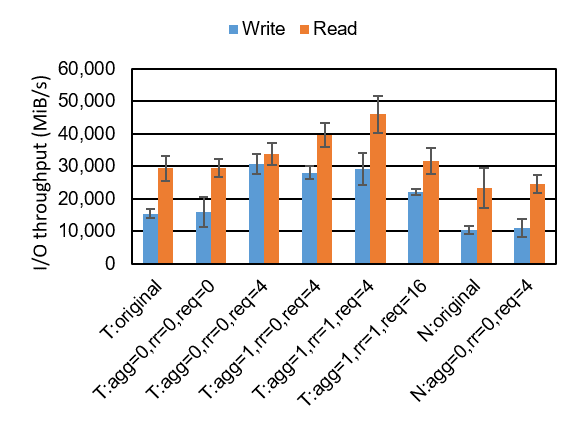
\includegraphics[width=1.0\textwidth]{IOR-results-ext.png}
 \subcaption{IOR benchmark}
 \label{fig:IOR_PERF}
\end{minipage}
%
\noindent
\begin{minipage}[t]{0.46\textwidth}
 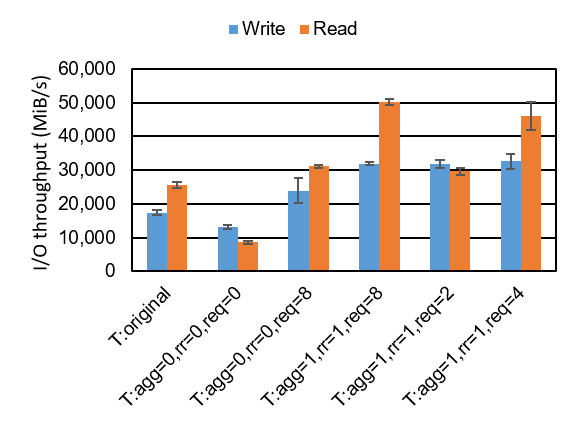
\includegraphics[width=1.0\textwidth]{hpio-results-ext.png}
 \subcaption{HPIO benchmark}
 \label{fig:HPIO_PERF}
\end{minipage}
\caption{
Benchmark results of the original MPI-IO and EARTH with several optimization
configurations by using (a) IOR and (b) HPIO}
\label{fig:IOR_HPIO_PERF}
\end{figure}
%

The original MPI-IO operations with and without two-phase I/O represented by
"{\tt T:original}" and "{\tt N:original}" show low performance in both read and write
operations in the IOR runs and the same situation is observed
for the "{\tt T:original}" case in the HPIO runs.
EARTH with full optimization in aggregator layout and I/O request throttling
and stepwise data aggregation outperformed other cases by setting four requests per step
({\tt T:agg=1,rr=1,req=4}) in the IOR runs and eight requests per step
({\tt T:agg=1,rr=1,req=8}) in the HPIO runs.
However, performance was degraded by changing the number of requests per step
or deactivating aggregator layout optimization.
Although we have learned optimization effects through such empirical benchmark runs,
it has not been clear about the performance impact of the optimization configuration
on I/O nodes and the LFS.

\subsection{Analysis of OSS stats files}

Figure~\ref{fig:IOR_OST_IO_STATS} shows the mean values of
{\tt req\_qdepth}, {\tt req\_waittime}, and {\tt req\_active} obtained from OSSes
during I/O operations at the IOR benchmark run.
%
\begin{figure}[htb]
\centering
\begin{minipage}[t]{0.88\textwidth}
 \centering
 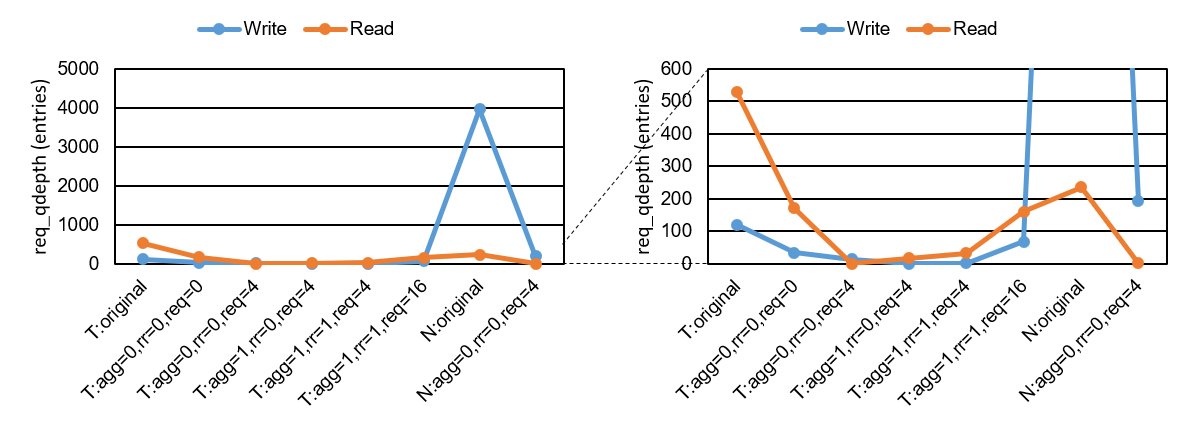
\includegraphics[width=1.0\textwidth]{IOR-ost_io_stats-qdepth-ext-dual.png}
 \subcaption{{\tt req\_qdepth}}
 \label{fig:IOR_req_qdepth}
\end{minipage}
%
\noindent
\begin{minipage}[t]{0.88\textwidth}
 \centering
 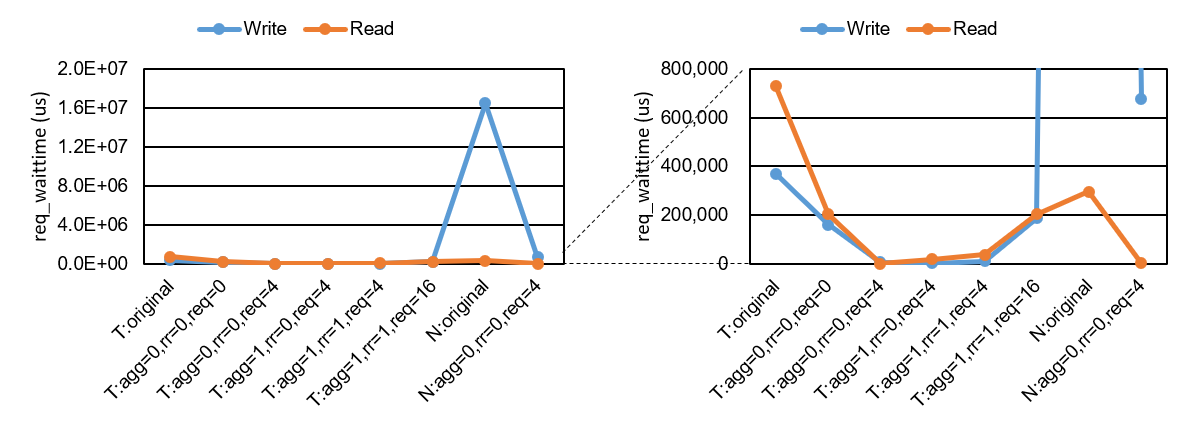
\includegraphics[width=1.0\textwidth]{IOR-ost_io_stats-waittime-ext-dual.png}
 \subcaption{{\tt req\_waittime}}
 \label{fig:IOR_req_waittime}
\end{minipage}
%
\noindent
\begin{minipage}[t]{0.4\textwidth}
 \centering
 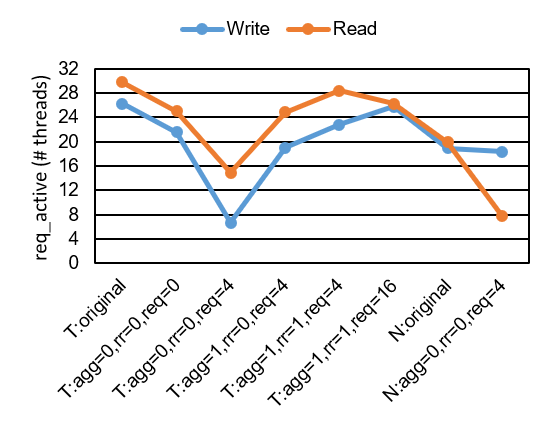
\includegraphics[width=1.0\textwidth]{IOR-ost_io_stats-active-ext.png}
 \subcaption{{\tt req\_active}}
 \label{fig:IOR_req_active}
\end{minipage}
%
\caption{Mean stats values obtained from OSSes using our analysis framework
during the IOR benchmark run}
\label{fig:IOR_OST_IO_STATS}
\end{figure}
%
The original case had the largest number of requests in a request queue
as shown in Fig.~\ref{fig:IOR_OST_IO_STATS}\subref{fig:IOR_req_qdepth}.
Fig.~\ref{fig:IOR_OST_IO_STATS}\subref{fig:IOR_req_waittime}
tells that this case also took the longest time to proceed requests.
Besides, Fig.~\ref{fig:IOR_OST_IO_STATS}\subref{fig:IOR_req_active} shows
the highest number of I/O threads in the original case.
Note that the maximum number of threads at each OSS of the LFS was 32
at the K computer.
Through the observed results, it has turned out that the original case was not
suited for I/O request processing at OSSes.

While the EARTH use case with good I/O performance ({\tt T:agg=1,rr=1,req=4})
showed quite a small number of requests in the queue as shown in
Fig.~\ref{fig:IOR_OST_IO_STATS}\subref{fig:IOR_req_qdepth}.
Fig.~\ref{fig:IOR_OST_IO_STATS}\subref{fig:IOR_req_waittime} also gives
the fact that this case took quite short times to process I/O requests.
Besides, Fig.~\ref{fig:IOR_OST_IO_STATS}\subref{fig:IOR_req_active}
tells us a high number of I/O threads was active for this case.

Figure~\ref{fig:HPIO_OST_IO_STATS} shows the same statistics obtained
in the HPIO benchmark run.
%
\begin{figure}[htb]
\centering
\begin{minipage}[t]{0.44\textwidth}
 \centering
 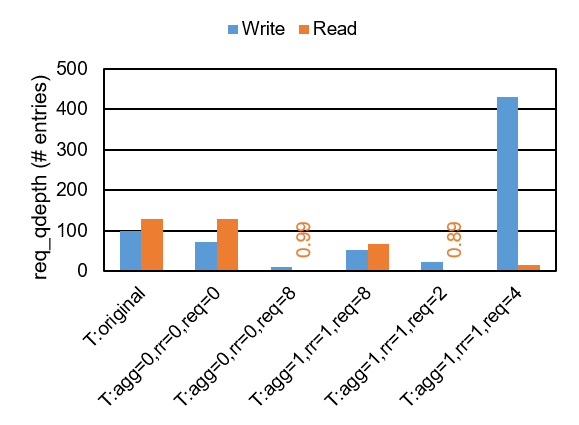
\includegraphics[width=1.0\textwidth]{hpio-ost_io_stats-qdepth-ext.png}
 \subcaption{{\tt req\_qdepth}}
 \label{fig:HPIO_req_qdepth}
\end{minipage}
%
\noindent
\begin{minipage}[t]{0.44\textwidth}
 \centering
 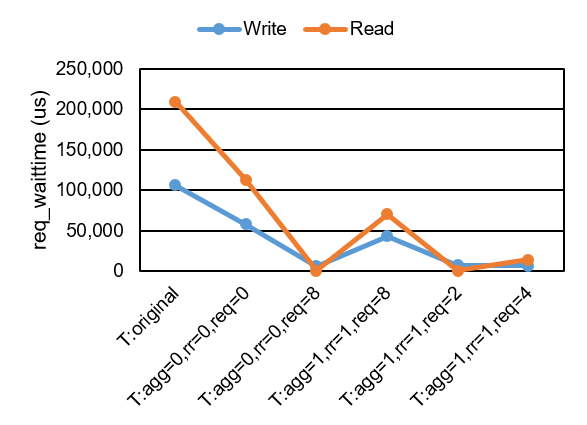
\includegraphics[width=1.0\textwidth]{hpio-ost_io_stats-waittime-ext.png}
 \subcaption{{\tt req\_waittime}}
 \label{fig:HPIO_req_waittime}
\end{minipage}
%
\noindent
\begin{minipage}[t]{0.44\textwidth}
 \centering
 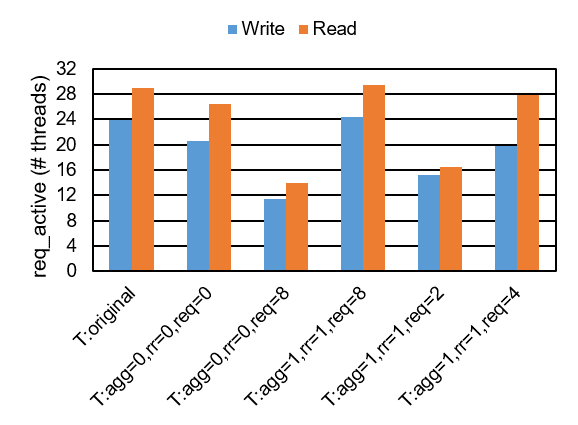
\includegraphics[width=1.0\textwidth]{hpio-ost_io_stats-active-ext.png}
 \subcaption{{\tt req\_active}}
 \label{fig:HPIO_req_active}
\end{minipage}
%
\caption{Mean stats values obtained from OSSes using our analysis framework
during the HPIO benchmark run}
\label{fig:HPIO_OST_IO_STATS}
\end{figure}
%
Similar to the IOR run, the original case was not good compared
with the EARTH case with good optimization configuration
indicated by "{\tt T:agg=1,rr=1,req=8}."

\subsection{Bandwidth utilization and waiting times in data transfers on Tofu interconnects of I/O nodes}

Figure~\ref{fig:IOR_ION_TOFU_BWU_WAIT_TIME} shows mean values of
(a) the peak bandwidth utilization ratios and
(b) the maximum waiting times in data transfers on links of used I/O nodes.
%
\begin{figure}[htb]
\centering
\begin{minipage}[t]{0.48\textwidth}
 \centering
 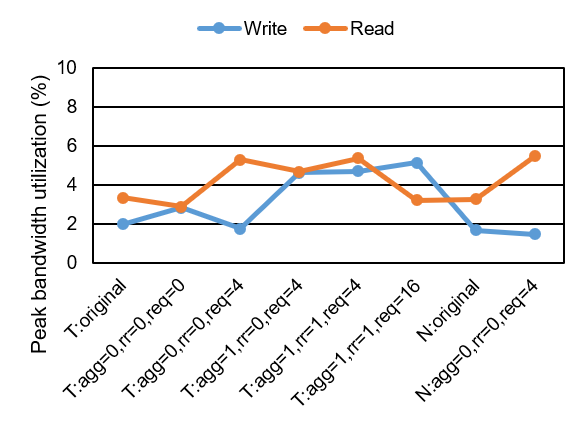
\includegraphics[width=1.0\textwidth]{IOR-bwu-IO-nodes-ext.png}
 \subcaption{Bandwidth utilization}
 \label{fig:IOR_ION_TOFU_BW_UTIL}
\end{minipage}
%
\noindent
\begin{minipage}[t]{0.48\textwidth}
 \centering
 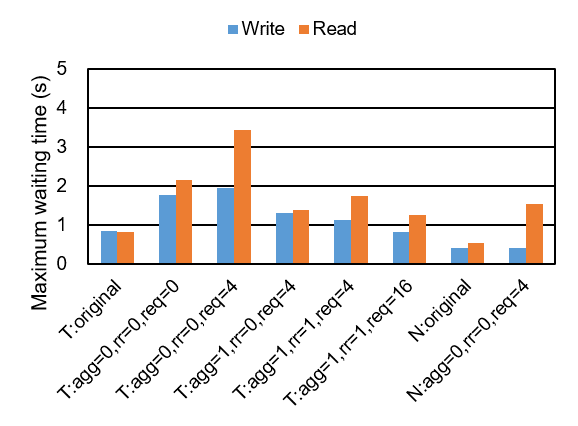
\includegraphics[width=1.0\textwidth]{IOR-zero_credit_sec-IO-nodes-ext.png}
 \subcaption{Waiting time in data transfer}
 \label{fig:IOR_ION_TOFU_WAIT_TIME}
\end{minipage}
\caption{
Mean values for data transfers on the Tofu interconnects among used I/O nodes
during the IOR benchmark run}
\label{fig:IOR_ION_TOFU_BWU_WAIT_TIME}
\end{figure}
%

Concerning bandwidth utilization shown in
Fig.~\ref{fig:IOR_ION_TOFU_BWU_WAIT_TIME}\subref{fig:IOR_ION_TOFU_BW_UTIL},
the original MPI-IO case shows the lowest utilization, while the full set of EARTH 
optimizations such as “{\tt T:agg=1,rr=1,req=4}” lead to higher bandwidth utilization
relative to other cases.
By considering effectiveness in data transfers among I/O nodes via Tofu interconnects,
a higher utilization is preferable.
In this context, the above optimized case was suitable for I/O optimization.

Fig.~\ref{fig:IOR_ION_TOFU_BWU_WAIT_TIME}\subref{fig:IOR_ION_TOFU_WAIT_TIME}
tells us that the enhanced implementation
without aggregator layout optimization indicated by “{\tt T:agg=0,rr=0,req=4}”
took the longest times.
It is also noted that this case also performed the lowest bandwidth utilization
in write operations as shown in
Fig.~\ref{fig:IOR_ION_TOFU_BWU_WAIT_TIME}\subref{fig:IOR_ION_TOFU_BW_UTIL}.
It is remarked that the lack of aggregator layout optimization in the EARTH case
led to a negative impact in data transfers on Tofu interconnects among I/O nodes.

In a similar way, Fig.~\ref{fig:HPIO_ION_TOFU_BWU_WAIT_TIME} shows
bandwidth utilization ratios and waiting times in data transfers
on Tofu links of used I/O nodes at the HPIO benchmark run.
%
\begin{figure}[htb]
\centering
\begin{minipage}[t]{0.48\textwidth}
 \centering
 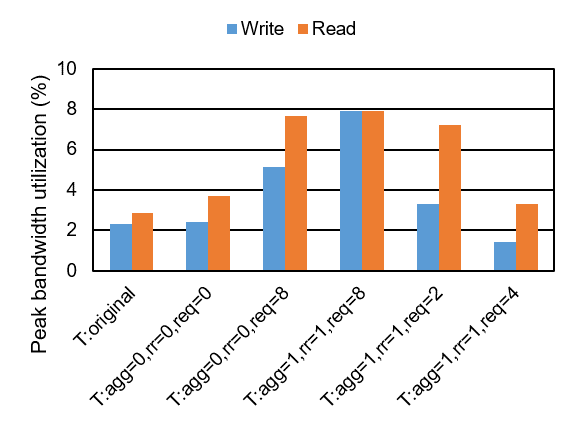
\includegraphics[width=0.98\textwidth]{hpio-bwu-IO-nodes-ext.png}
 \subcaption{Bandwidth utilization}
 \label{fig:HPIO_ION_TOFU_BW_UTIL}
\end{minipage}
%
\noindent
\begin{minipage}[t]{0.48\textwidth}
 \centering
 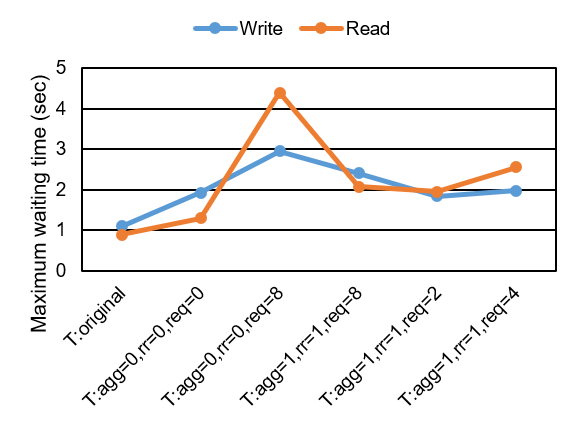
\includegraphics[width=0.98\textwidth]{hpio-zero_credit_sec-IO-nodes-ext.png}
 \subcaption{Waiting time in data transfer}
 \label{fig:HPIO_ION_TOFU_WAIT_TIME}
\end{minipage}
\caption{
Mean values for data transfers on the Tofu interconnects among used I/O nodes
during the HPIO benchmark run}
\label{fig:HPIO_ION_TOFU_BWU_WAIT_TIME}
\end{figure}
%
The EARTH case with the best configuration ({\tt T:agg=1,rr=1,req=8}) also
outperformed other cases in
Fig.~\ref{fig:HPIO_ION_TOFU_BWU_WAIT_TIME}\subref{fig:HPIO_ION_TOFU_BW_UTIL}.
This case also showed shorter times in both read and write operations
among the EARTH cases in
Fig.~\ref{fig:HPIO_ION_TOFU_BWU_WAIT_TIME}\subref{fig:HPIO_ION_TOFU_WAIT_TIME}.

\subsection{Load balancing in I/O throughput at OSTs}

Figure~\ref{fig:IOR_OST_BW_HMAP_WR} shows write bandwidth heat-maps
among the 192 OSTs during the IOR benchmark runs.
%
\begin{figure}[htb]
%% \centering
\begin{minipage}[t]{0.06\textwidth}
 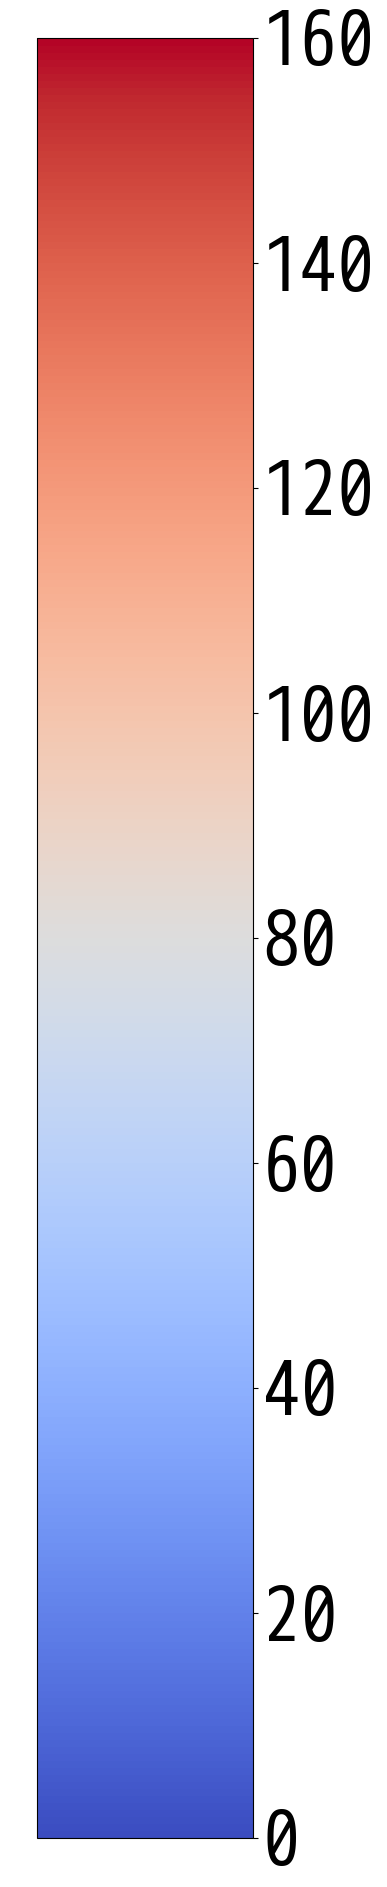
\includegraphics[width=0.98\textwidth,height=0.14\textheight]{hmap-colorbar-mod2.png}
\end{minipage}
%
\noindent
\begin{minipage}[t]{0.3\textwidth}
 \centering
 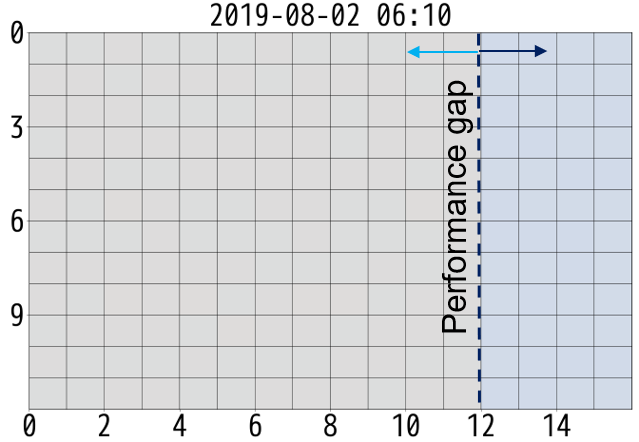
\includegraphics[width=0.98\textwidth]{IOR-OST_bw_hmap-TP-orig-write-mod.png}
 \subcaption{{\tt T:original}}
 \label{fig:IOR_OST_WR_ORIG}
\end{minipage}
%
\noindent
\begin{minipage}[t]{0.3\textwidth}
 \centering
 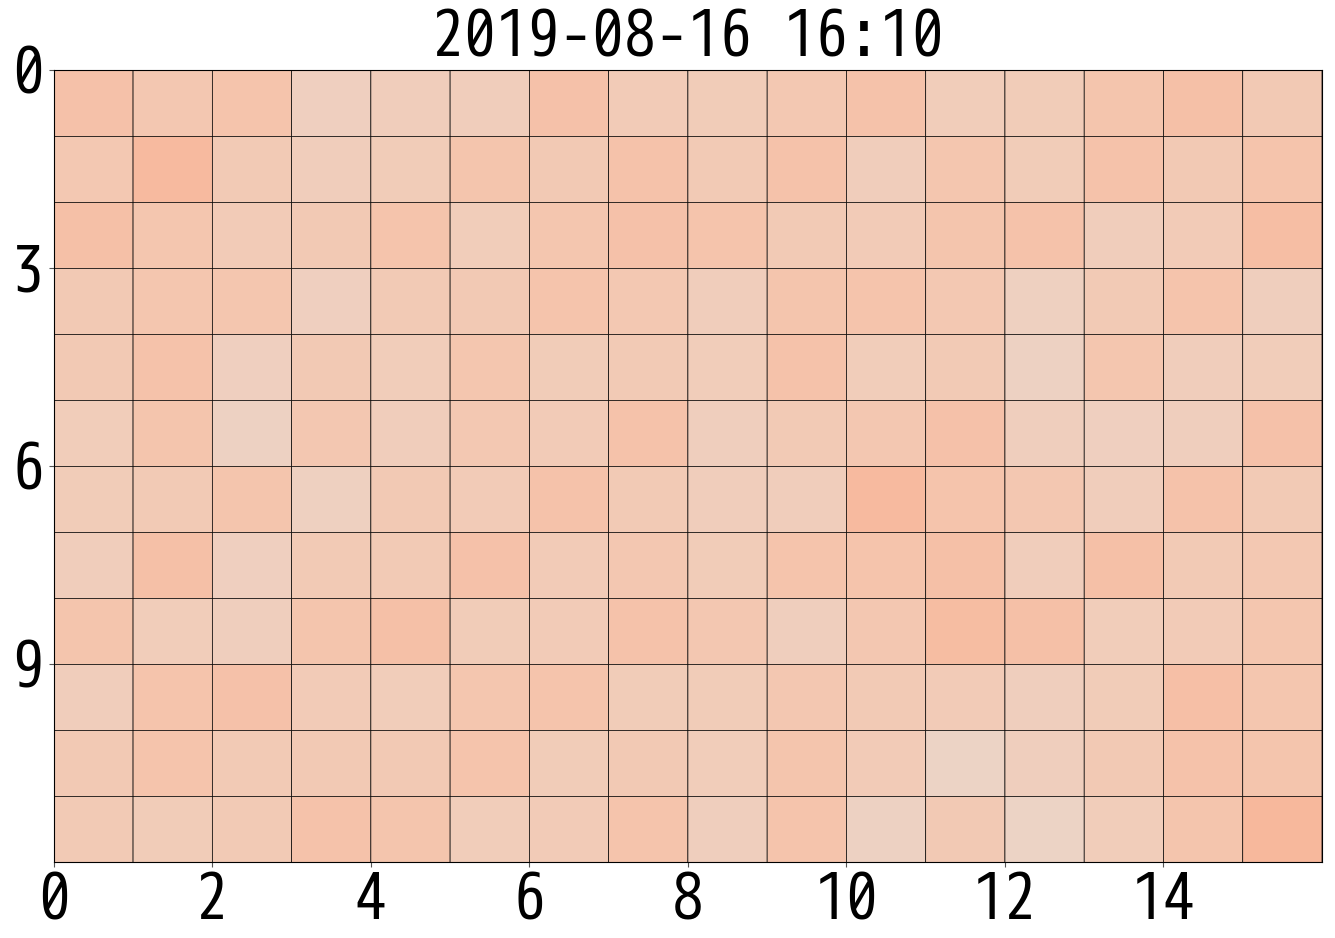
\includegraphics[width=0.98\textwidth]{IOR-OST_bw_hmap-TP-earth-agg0-rr0-req0-write-mod.png}
 \subcaption{{\tt T:agg=0,rr=0,req=0}}
 \label{fig:IOR_OST_WR_AGG0_RR0_REQ0}
\end{minipage}
%
\noindent
\begin{minipage}[t]{0.3\textwidth}
 \centering
 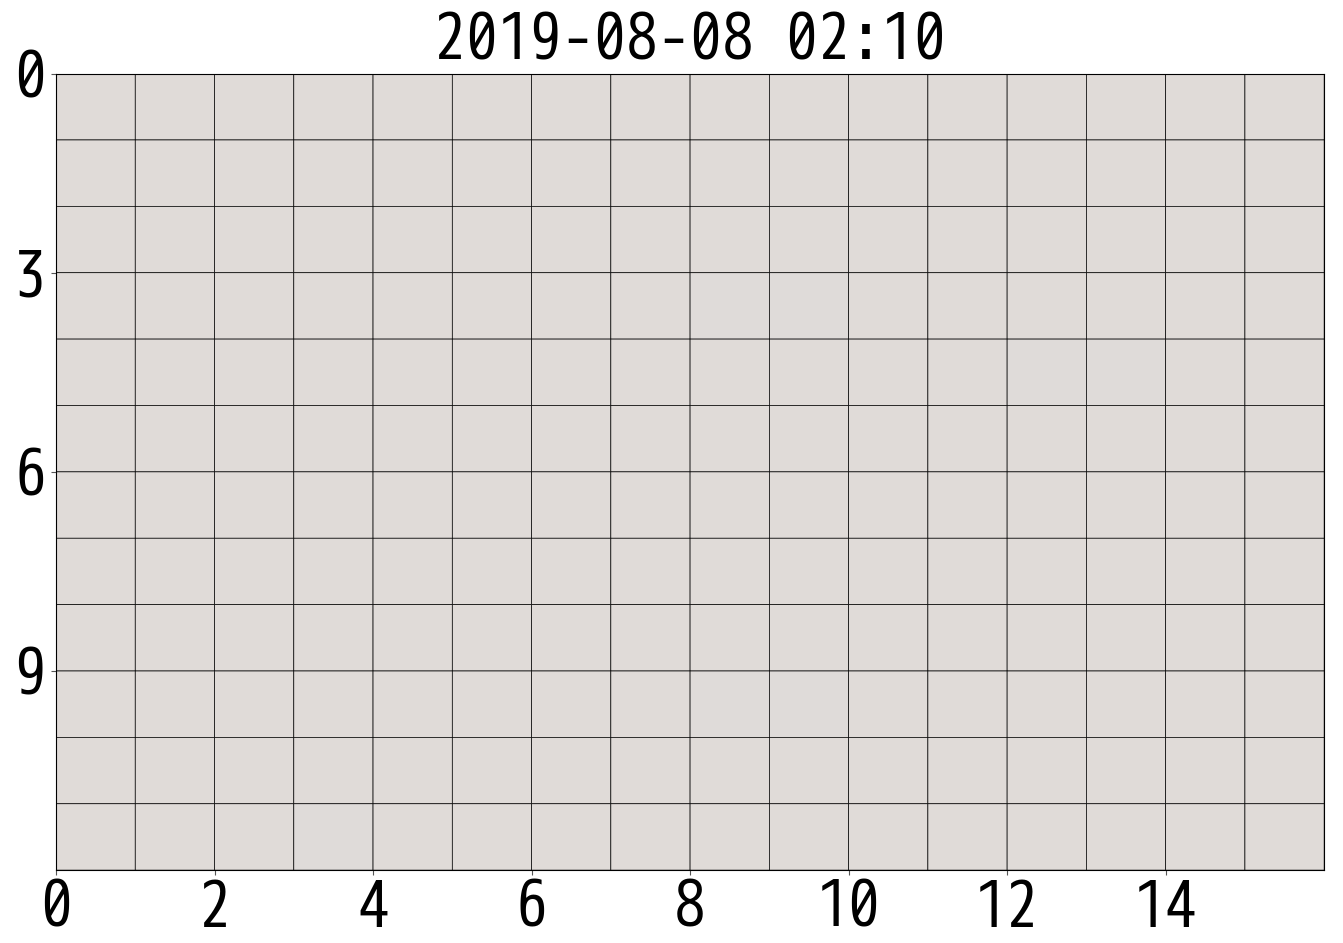
\includegraphics[width=0.98\textwidth]{IOR-OST_bw_hmap-TP-earth-agg1-rr1-req4-write-mod.png}
 \subcaption{{\tt T:agg=1,rr=1,req=4}}
 \label{fig:IOR_OST_WR_AGG1_RR1_REQ4}
\end{minipage}
%
\caption{Write bandwidth heat-maps for 192 OSTs during the IOR benchmark run}
\label{fig:IOR_OST_BW_HMAP_WR}
\end{figure}
%
Each heat-map showed write bandwidth of each OST ranging from 0 to 160 MiB/s,
where horizontal and vertical directions indicate subjected relative 2D positions
of used OSTs from the logical 3D layout of the K computer,
ranging from 0 to 15 and from 0 to 11 in horizontal and vertical directions, respectively.

In the original MPI-IO case in Fig.~\ref{fig:IOR_OST_BW_HMAP_WR}\subref{fig:IOR_OST_WR_ORIG},
we can see performance gaps among the left and right sides separated by
the dotted line.
Fig.~\ref{fig:IOR_OST_BW_HMAP_WR}\subref{fig:IOR_OST_WR_AGG0_RR0_REQ0}
also shows performance gaps among OSTs
because of imbalanced aggregator layout although the EARTH was used.
Both cases are not suitable because total I/O performance is limited
by the slowest OSTs in parallel I/O.
While the most optimized case in
Fig.~\ref{fig:IOR_OST_BW_HMAP_WR}\subref{fig:IOR_OST_WR_AGG1_RR1_REQ4}
shows a well-balanced situation in write throughput among OSTs.
In the context of parallel I/O characteristics, this case was suitable
to achieve I/O performance for the benchmark run.

Figure~\ref{fig:IOR_OST_BW_HMAP_RD} shows read bandwidth heat-maps
among the 192 OSTs at the IOR benchmark runs.
%
\begin{figure}[htb]
\begin{minipage}[t]{0.06\textwidth}
 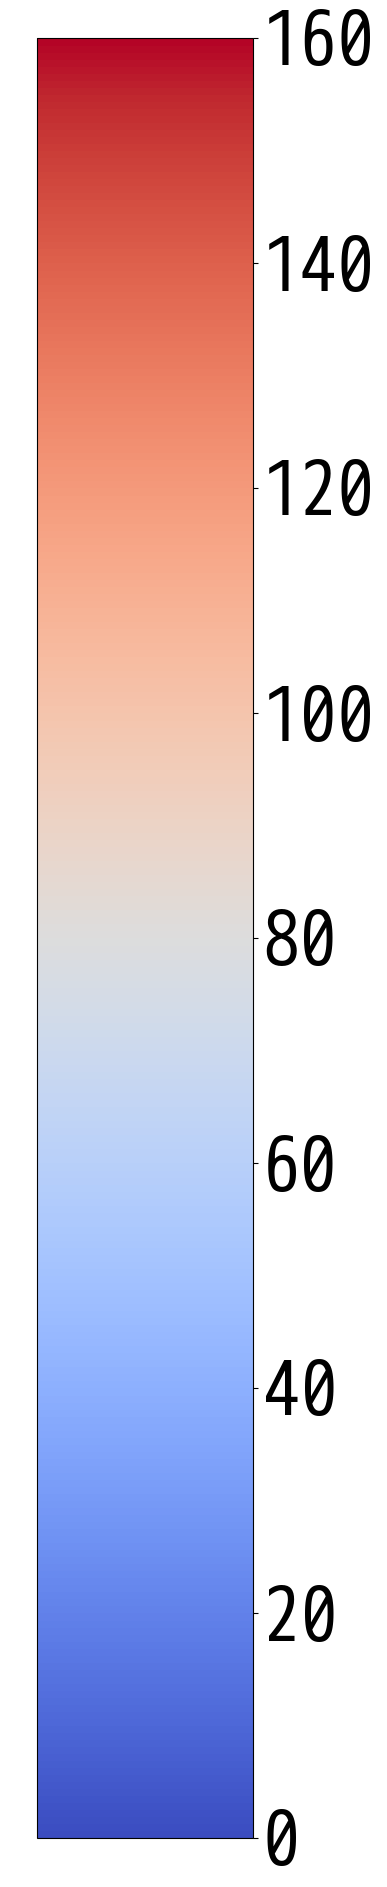
\includegraphics[width=0.98\textwidth,height=0.14\textheight]{hmap-colorbar-mod2.png}
\end{minipage}
%
\noindent
\begin{minipage}[t]{0.3\textwidth}
 \centering
 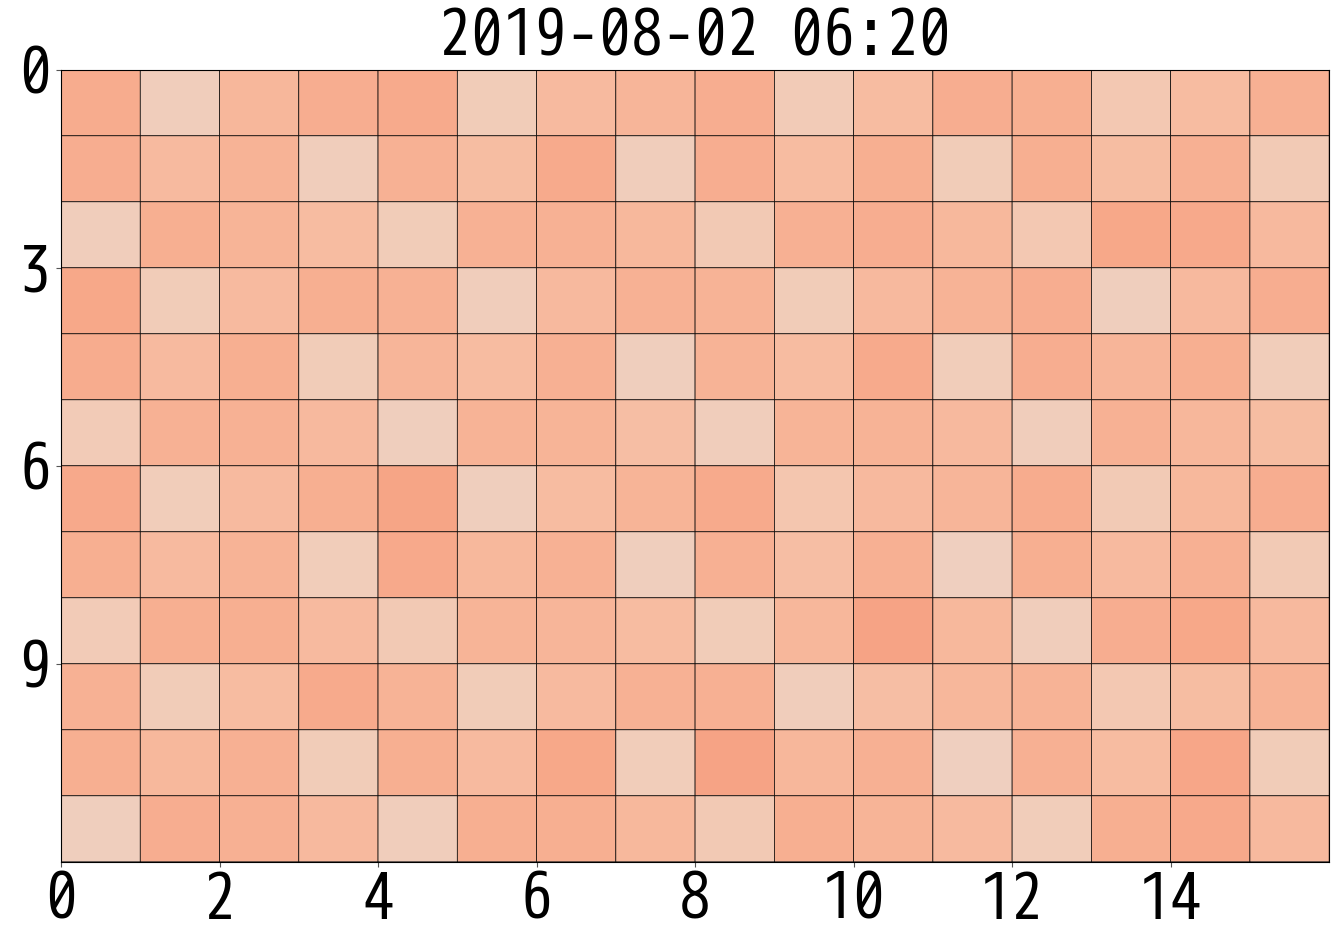
\includegraphics[width=0.98\textwidth]{IOR-OST_bw_hmap-TP-orig-read-mod.png}
 \subcaption{{\tt T:original}}
 \label{fig:IOR_OST_RD_ORIG}
\end{minipage}
%
\noindent
\begin{minipage}[t]{0.3\textwidth}
 \centering
 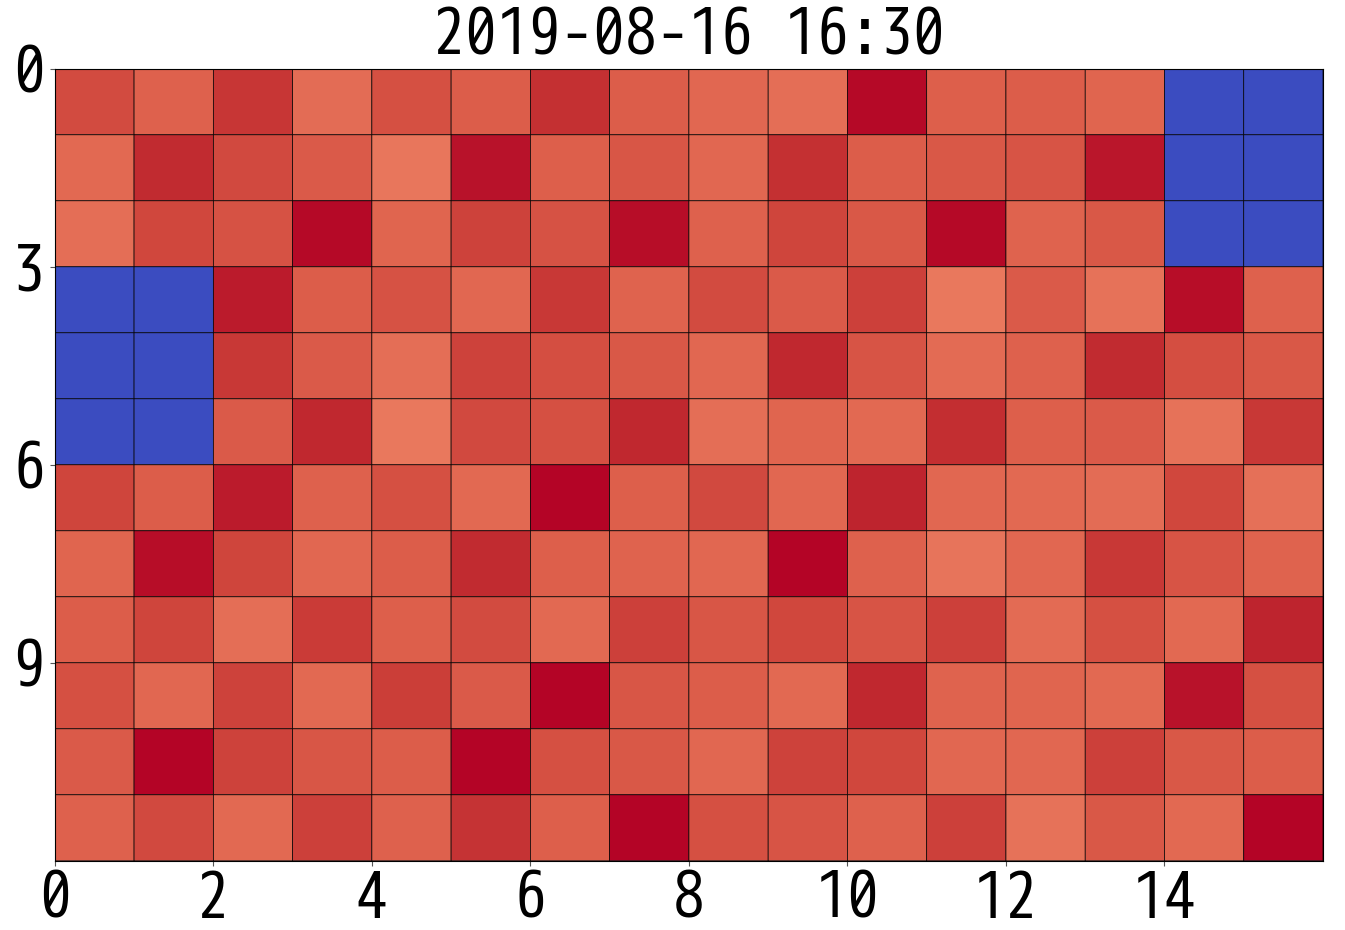
\includegraphics[width=0.98\textwidth]{IOR-OST_bw_hmap-TP-earth-agg0-rr0-req0-read-mod.png}
 \subcaption{{\tt T:agg=0,rr=0,req=0}}
 \label{fig:IOR_OST_RD_AGG0_RR0_REQ0}
\end{minipage}
%
\noindent
\begin{minipage}[t]{0.3\textwidth}
 \centering
 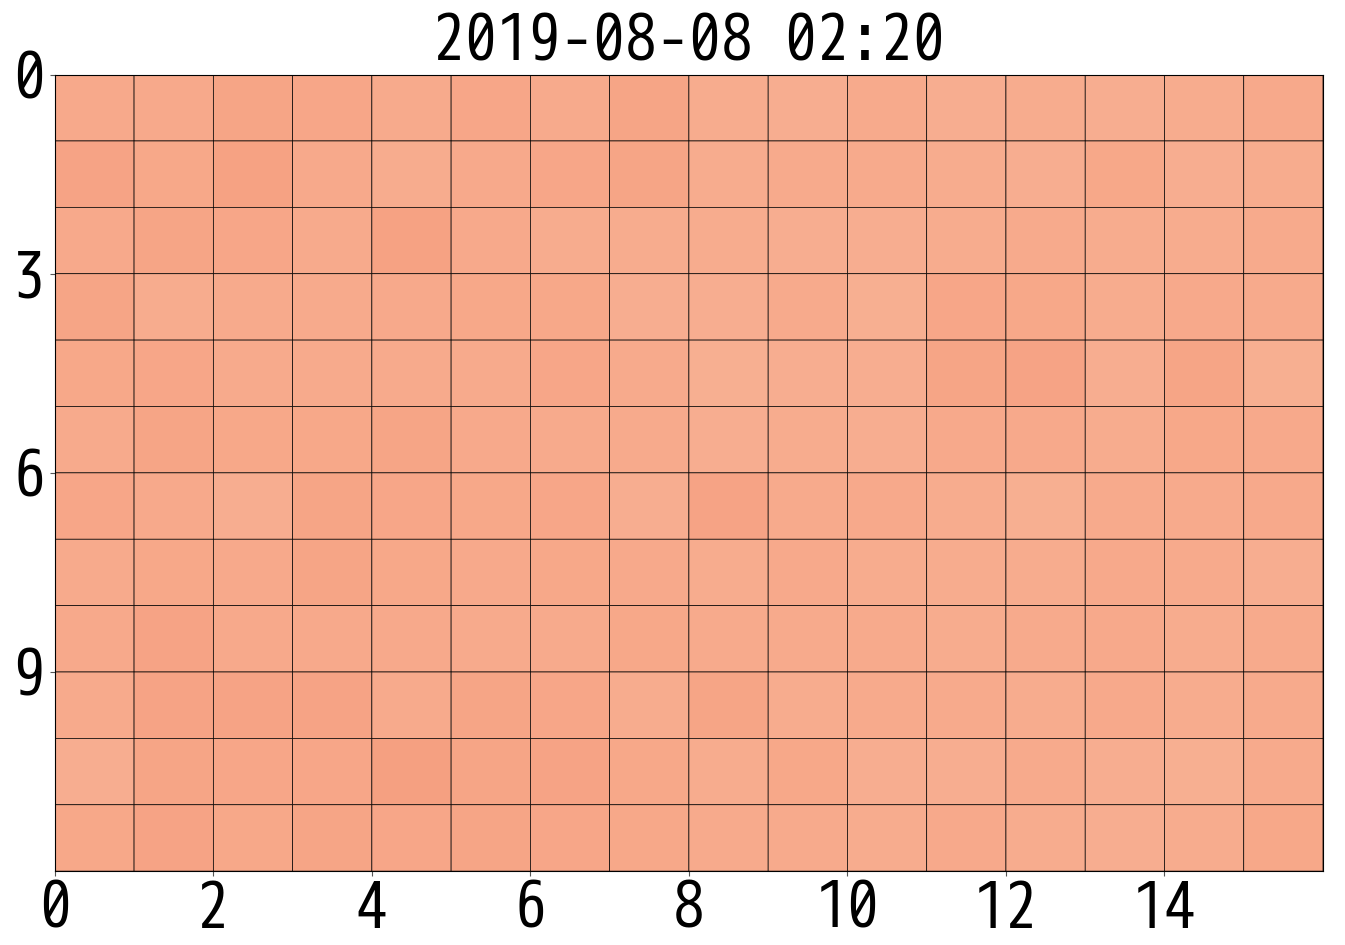
\includegraphics[width=0.98\textwidth]{IOR-OST_bw_hmap-TP-earth-agg1-rr1-req4-read-mod.png}
 \subcaption{{\tt T:agg=1,rr=1,req=4}}
 \label{fig:IOR_OST_RD_AGG1_RR1_REQ4}
\end{minipage}
%
\caption{Read bandwidth heat-maps for 192 OSTs during the IOR benchmark run}
\label{fig:IOR_OST_BW_HMAP_RD}
\end{figure}
%
Imbalanced bandwidth situation is observed in the original MPI-IO case shown in
Fig.~\ref{fig:IOR_OST_BW_HMAP_RD}\subref{fig:IOR_OST_RD_ORIG}
and the EARTH case without optimization shown
in Fig.~\ref{fig:IOR_OST_BW_HMAP_RD}\subref{fig:IOR_OST_RD_AGG0_RR0_REQ0}.
While well-balanced situation has been achieved in the EARTH case
with a good optimization configuration as shown in
Fig.~\ref{fig:IOR_OST_BW_HMAP_RD}\subref{fig:IOR_OST_RD_AGG1_RR1_REQ4},
which has led to high performance in collective I/O.

Write and read bandwidth heat-maps at the HPIO run are also shown in
Figures~\ref{fig:HPIO_OST_BW_HMAP_WR}
and \ref{fig:HPIO_OST_BW_HMAP_RD}, respectively.
%
\begin{figure}[htb]
\begin{minipage}[t]{0.06\textwidth}
 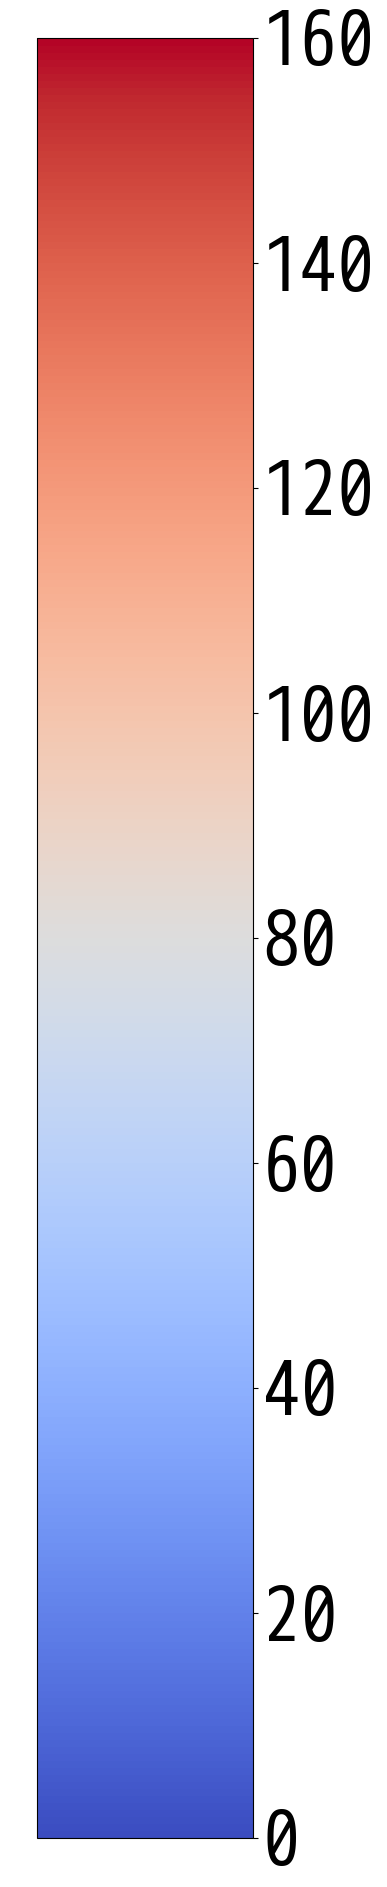
\includegraphics[width=0.98\textwidth,height=0.14\textheight]{hmap-colorbar-mod2.png}
\end{minipage}
%
\noindent
\begin{minipage}[t]{0.29\textwidth}
 \centering
 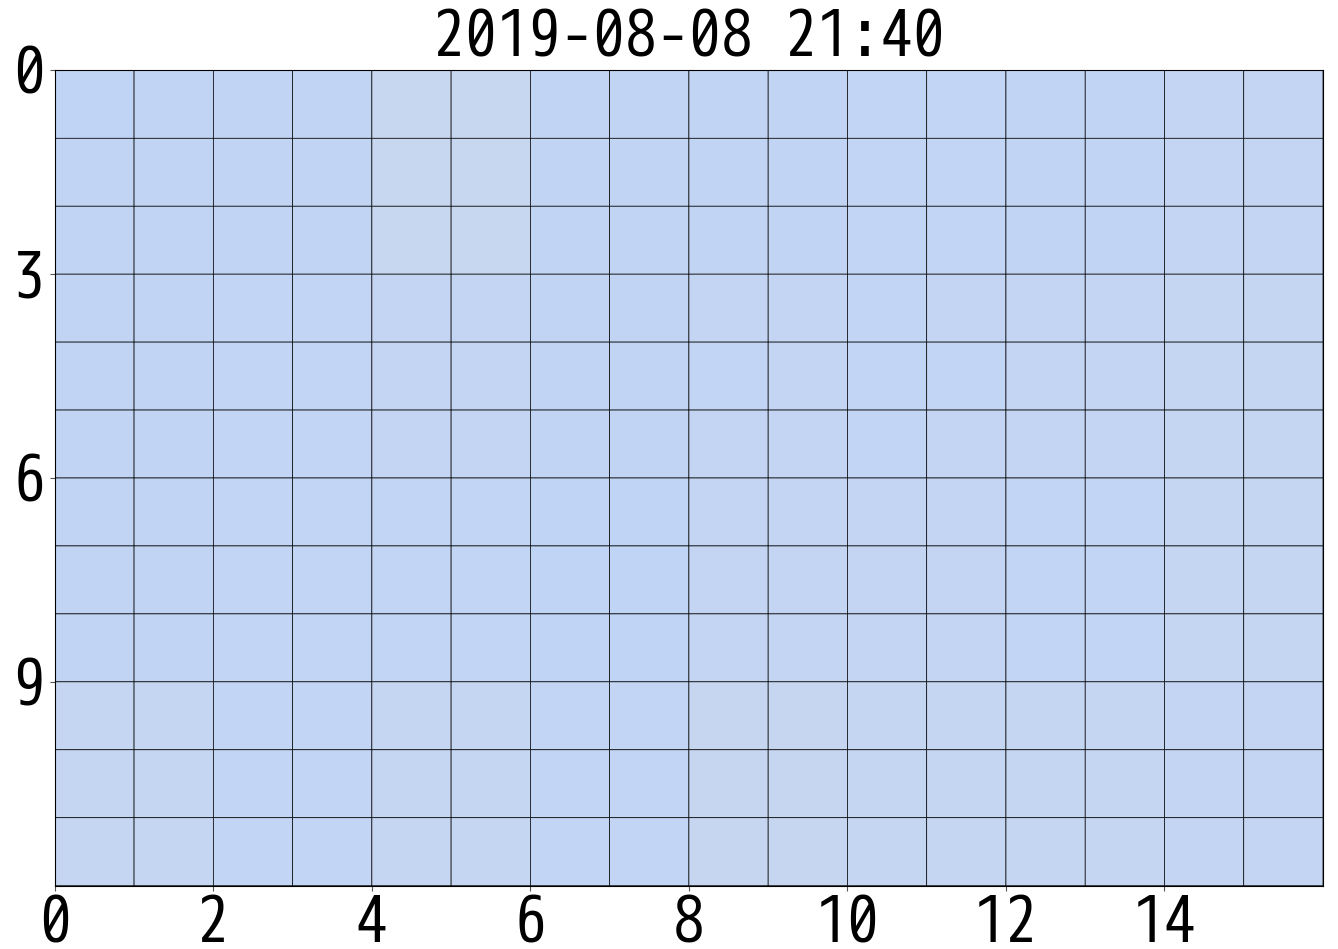
\includegraphics[width=0.96\textwidth]{hpio-OST_bw_hmap-orig-write-mod.png}
 \subcaption{{\tt T:original}}
\end{minipage}
%
\noindent
\begin{minipage}[t]{0.29\textwidth}
 \centering
 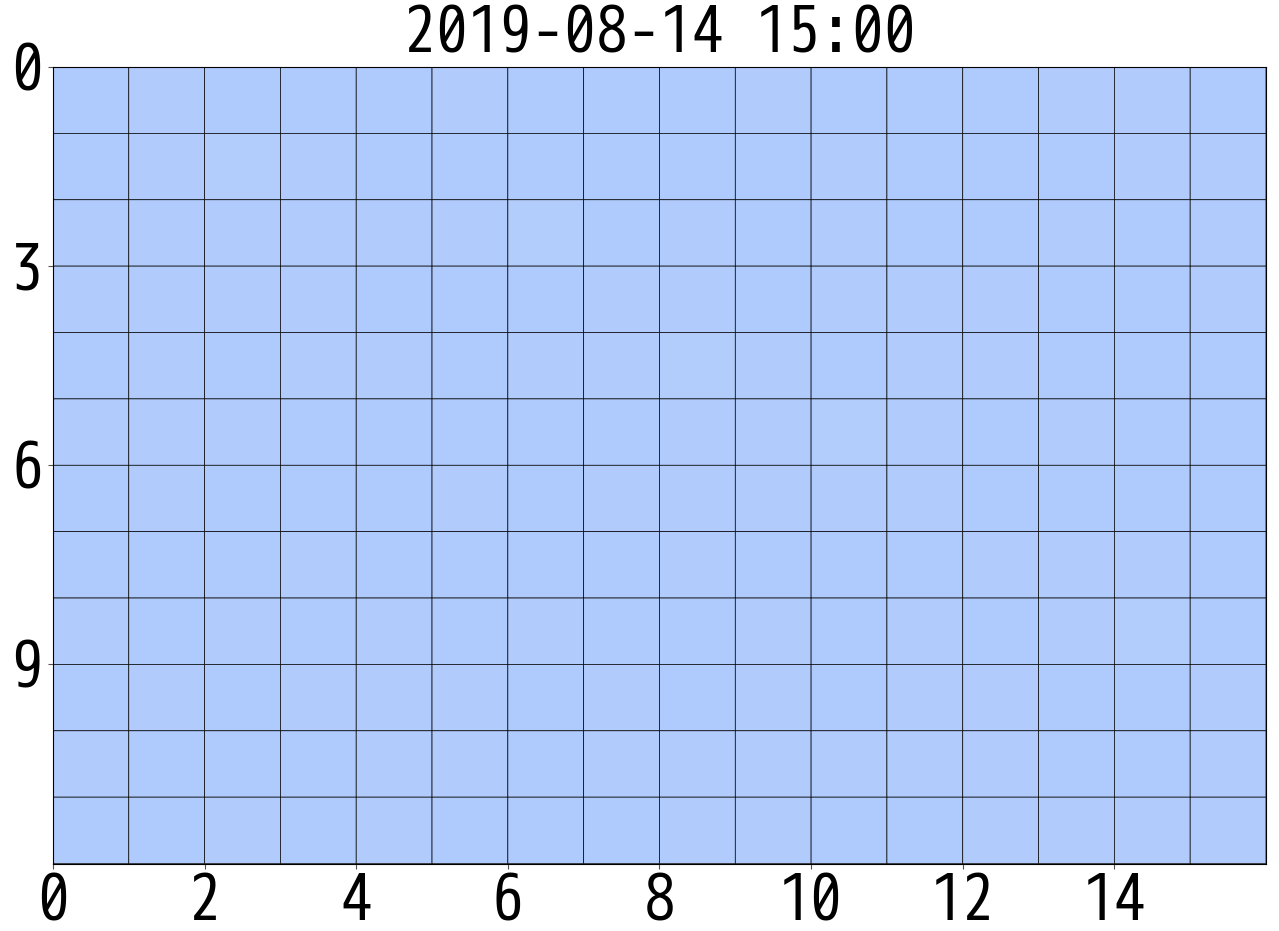
\includegraphics[width=0.96\textwidth]{hpio-OST_bw_hmap-earth-agg0-rr0-req8-write-mod.png}
 \subcaption{{\tt T:agg=0,rr=0,req=8}}
\end{minipage}
%
\noindent
\begin{minipage}[t]{0.31\textwidth}
 \centering
 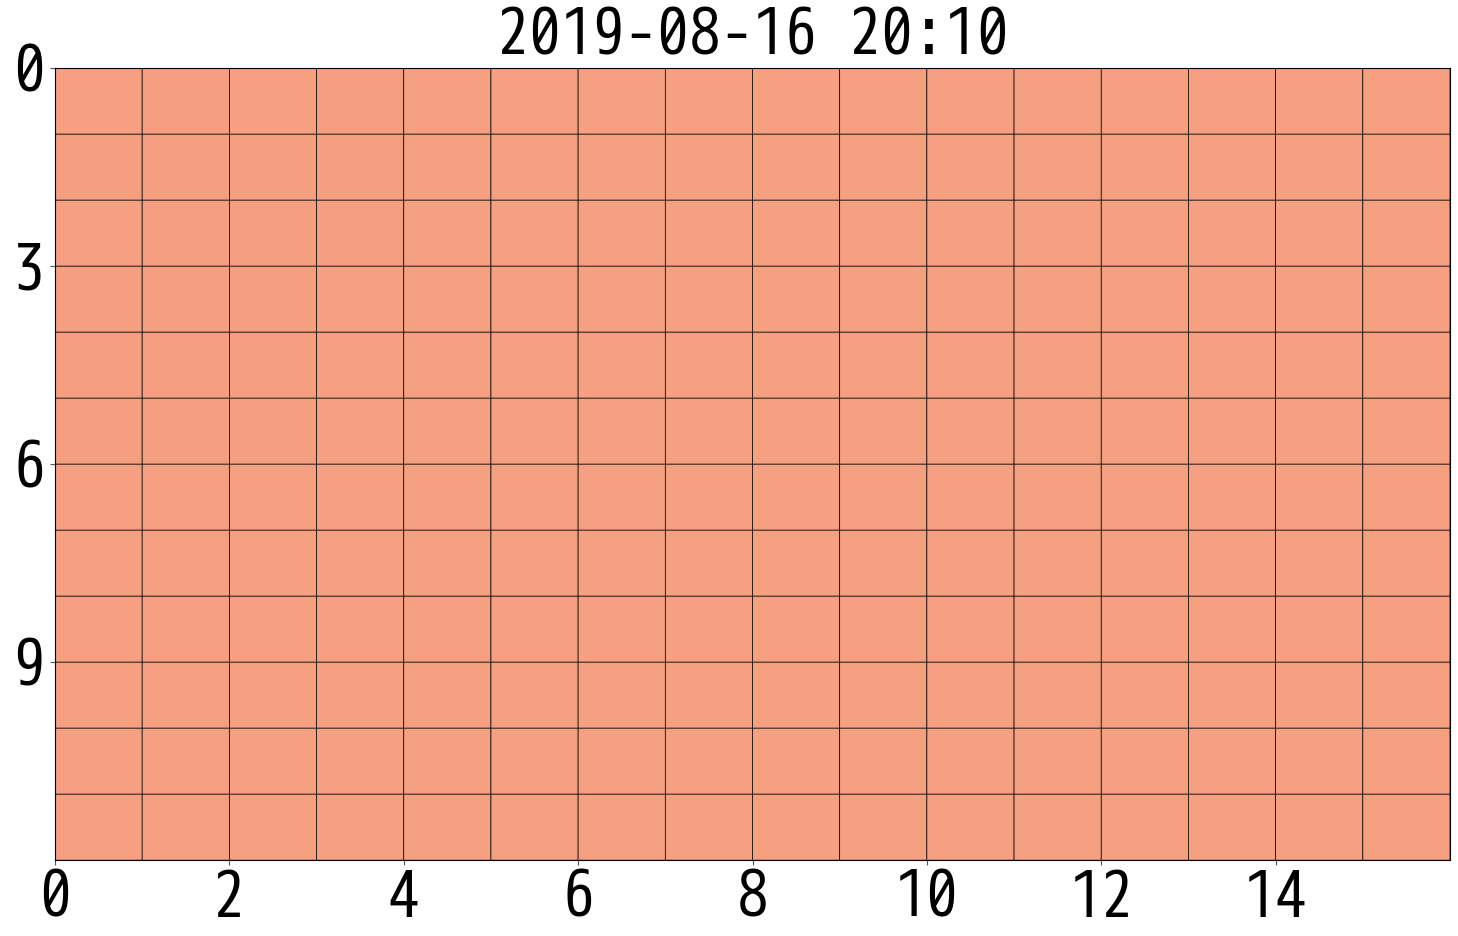
\includegraphics[width=1.0\textwidth]{hpio-OST_bw_hmap-earth-agg1-rr1-req8-write-mod.png}
 \subcaption{{\tt T:agg=1,rr=1,req=8}}
\end{minipage}
%
\caption{Write bandwidth heat-maps of used 192 OSTs at the HPIO benchmark run}
\label{fig:HPIO_OST_BW_HMAP_WR}
\end{figure}
%
\begin{figure}[tb]
\begin{minipage}[t]{0.06\textwidth}
 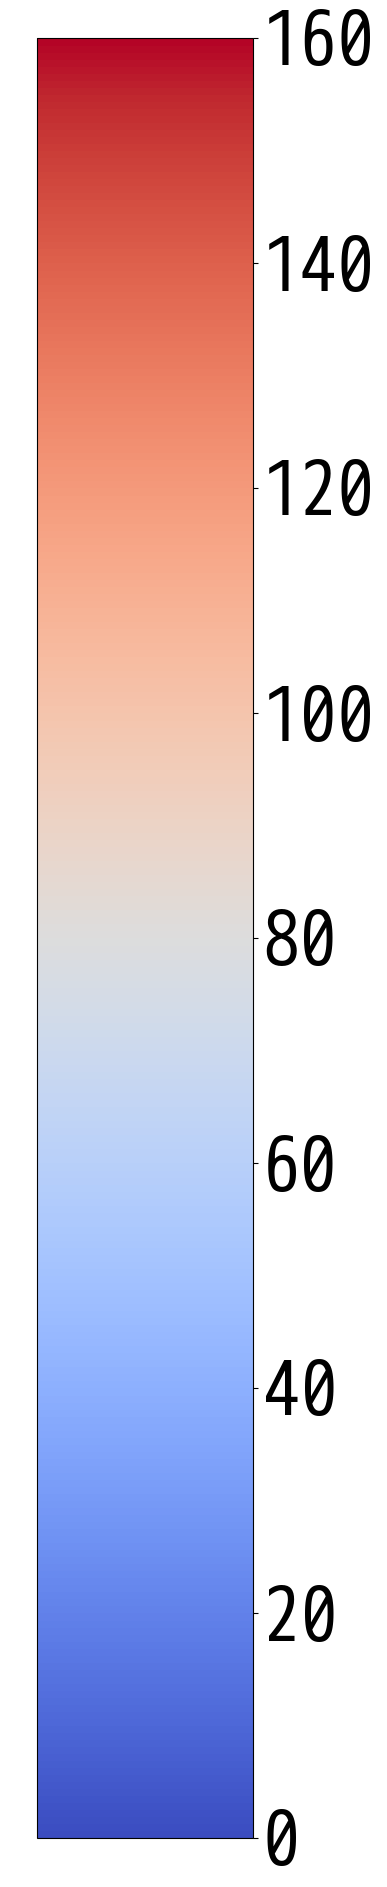
\includegraphics[width=0.98\textwidth,height=0.14\textheight]{hmap-colorbar-mod2.png}
\end{minipage}
%
\noindent
\begin{minipage}[t]{0.29\textwidth}
 \centering
 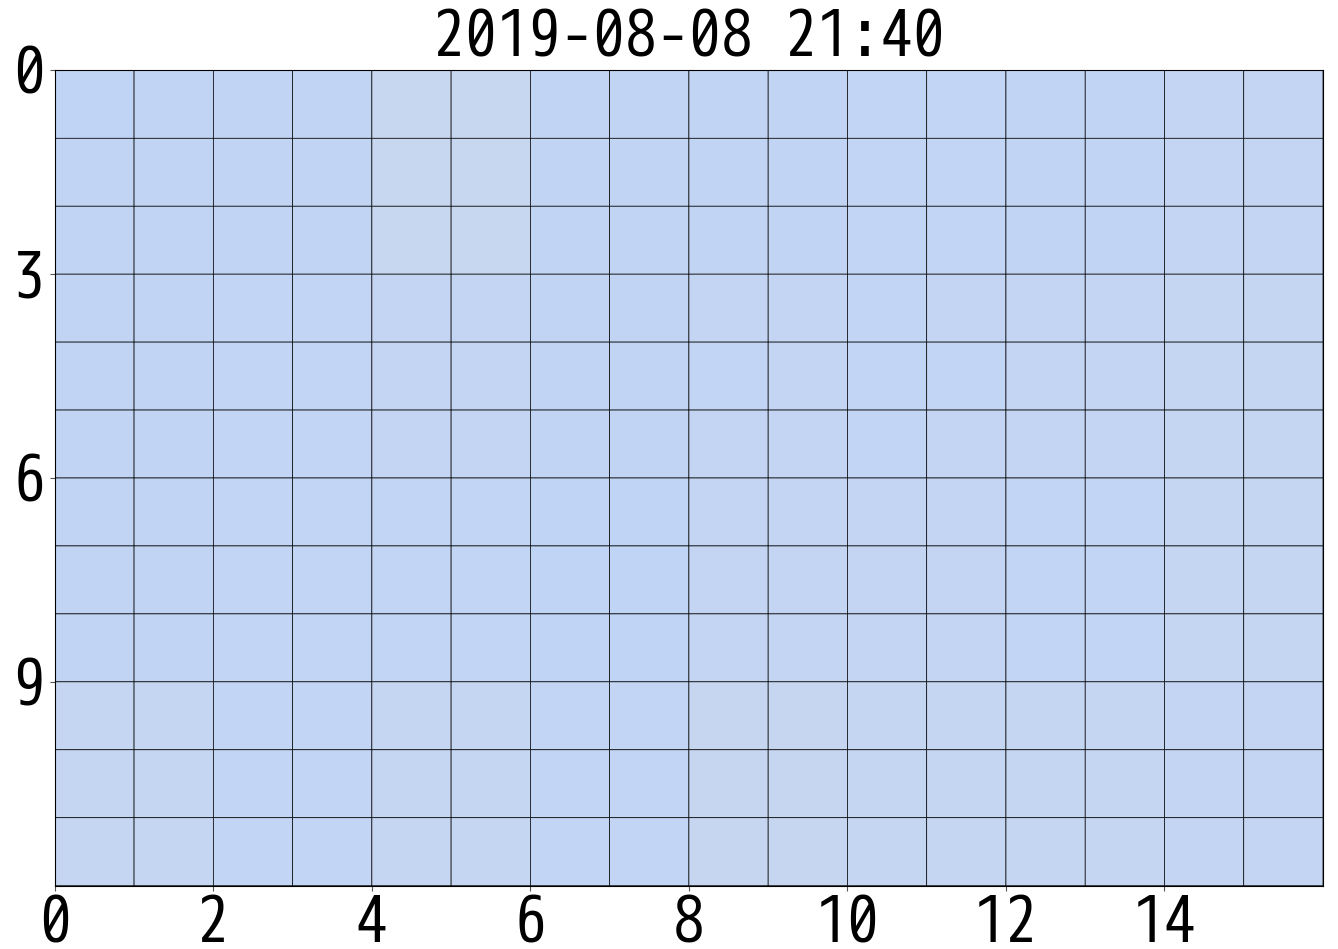
\includegraphics[width=0.96\textwidth]{hpio-OST_bw_hmap-orig-write-mod.png}
 \subcaption{{\tt T:original}}
\end{minipage}
%
\noindent
\begin{minipage}[t]{0.29\textwidth}
 \centering
 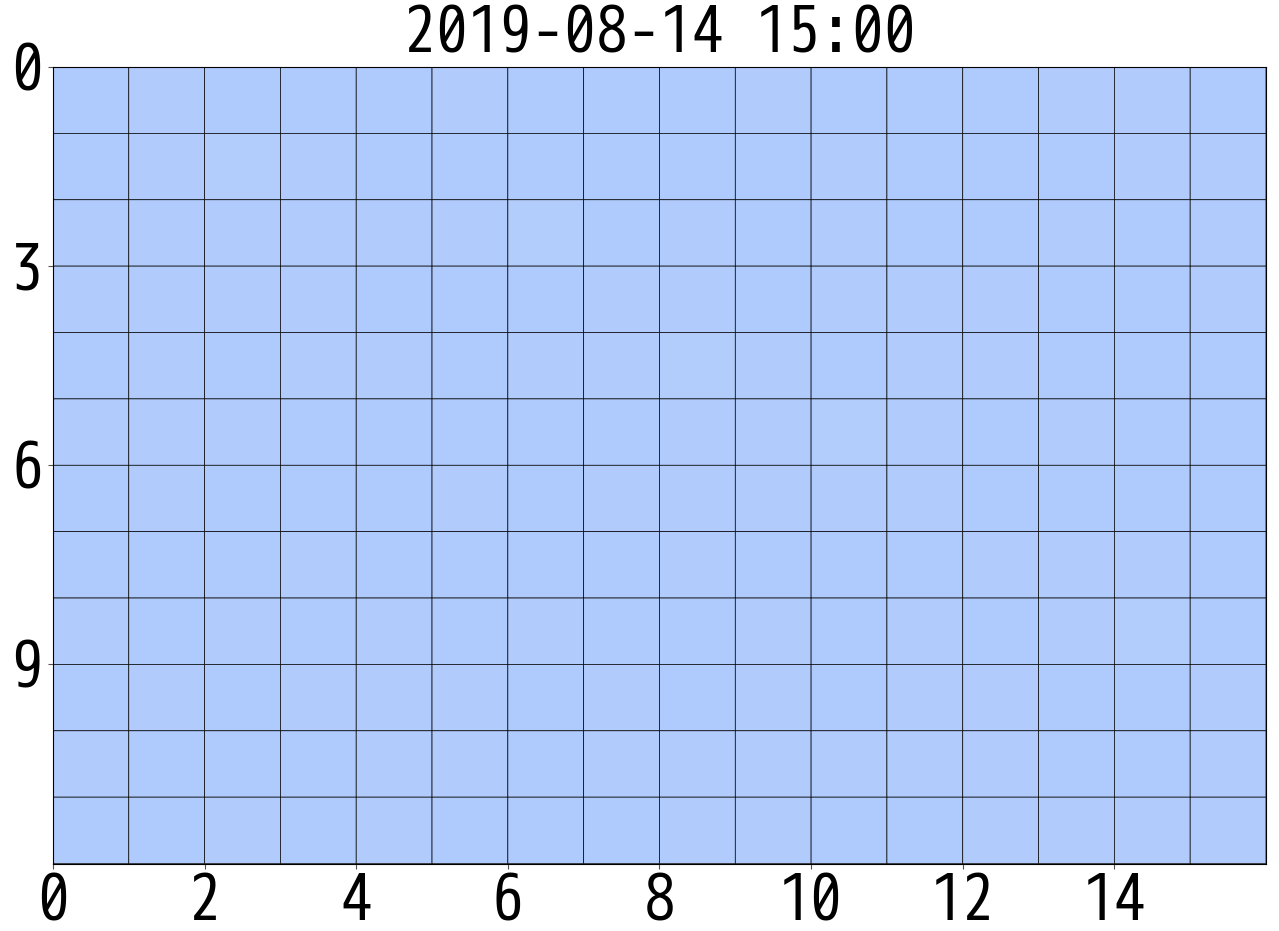
\includegraphics[width=0.96\textwidth]{hpio-OST_bw_hmap-earth-agg0-rr0-req8-write-mod.png}
 \subcaption{{\tt T:agg=0,rr=0,req=8}}
\end{minipage}
%
\noindent
\begin{minipage}[t]{0.31\textwidth}
 \centering
 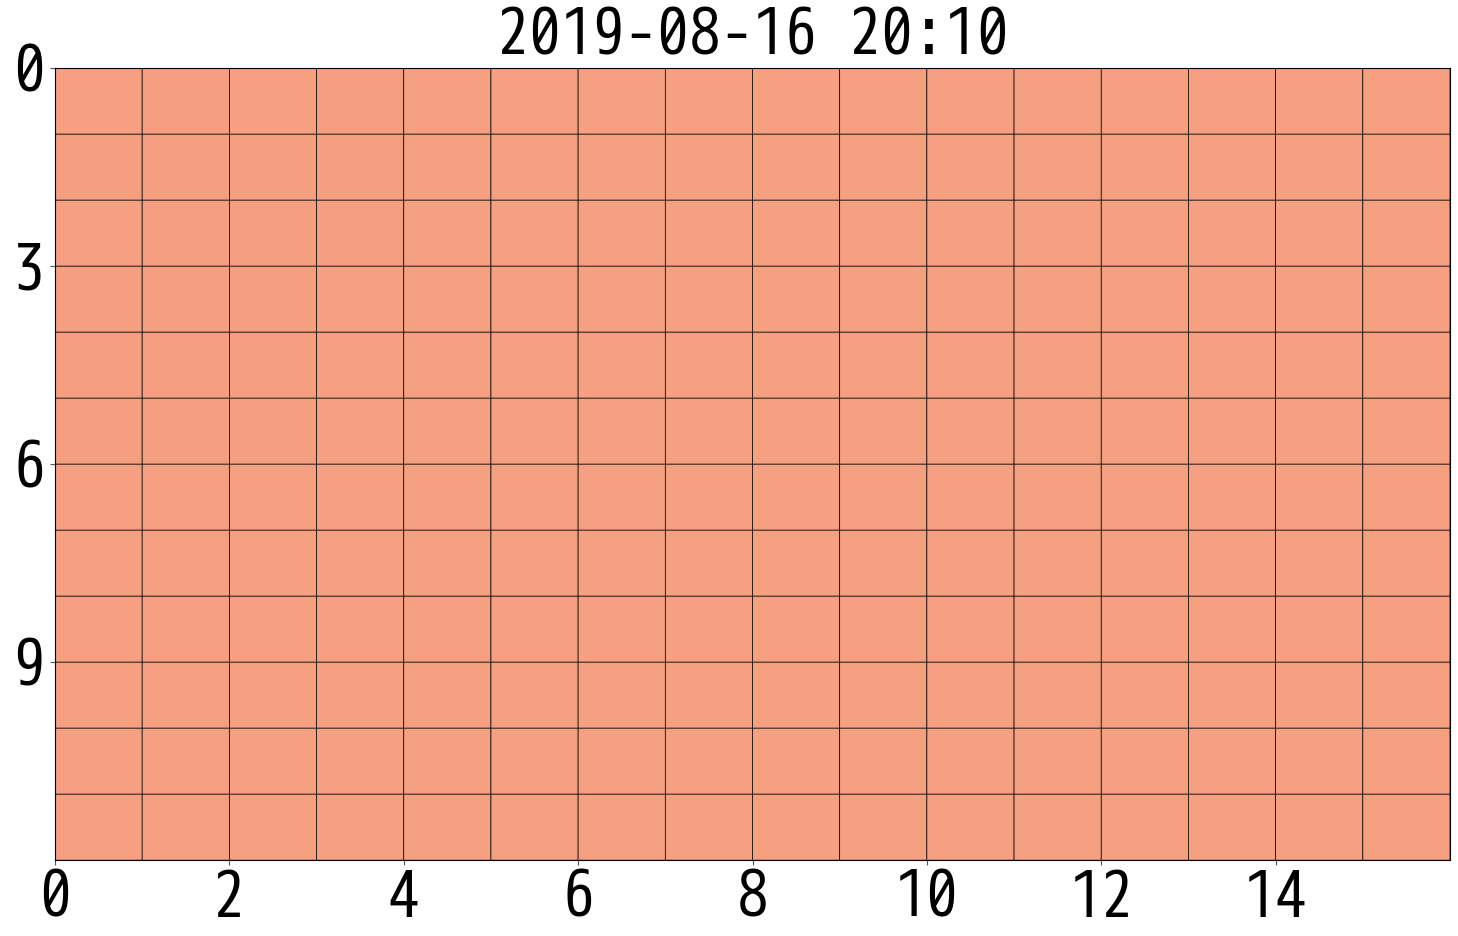
\includegraphics[width=1.0\textwidth]{hpio-OST_bw_hmap-earth-agg1-rr1-req8-write-mod.png}
 \subcaption{{\tt T:agg=1,rr=1,req=8}}
\end{minipage}
%
\caption{Read bandwidth heat-maps of used 192 OSTs at the HPIO benchmark run}
\label{fig:HPIO_OST_BW_HMAP_RD}
\end{figure}
%
In Fig.~\ref{fig:HPIO_OST_BW_HMAP_RD}, the EARTH case with insufficient configuration
({\tt T:agg=0,rr=0,req=8}) showed lower performance compared with the original MPI-IO case.
Meanwhile, a full set of the three optimizations in the EARTH case
({\tt T:agg=1,rr=1,req=8}) achieved the highest I/O throughput at every used OST. 
Read bandwidth heatmaps in Fig.~\ref{fig:HPIO_OST_BW_HMAP_RD} show
the highest I/O throughput in the insufficient optimization configuration
({\tt T:agg=0,rr=0,req=8}), followed by the original MPI-IO case
and the full optimization configuration case.
However, the insufficient configuration case has performed the longest waiting time
in the Tofu interconnects among the used I/O nodes as shown in
Fig.~\ref{fig:HPIO_ION_TOFU_BWU_WAIT_TIME}\subref{fig:HPIO_ION_TOFU_WAIT_TIME}
and thus high I/O bandwidth could not be achieved in this configuration.

\section{Conclusions}
\label{sec:CONCLUSIONS}

We have built a holistic log data analysis framework to characterize I/O activities
at the LFS and data transfers through the Tofu interconnects of I/O nodes
in I/O optimization at the K computer.
The proposed framework utilizes the bandwidth status of the Tofu links
among I/O nodes and performance metrics of log data generated at the LFS and I/O nodes.
The holistic analysis of data transfer activities on the Tofu links among I/O nodes
and I/O activities on the LFS provides useful information in I/O performance tuning.

Two I/O benchmark runs showed distinct differences in I/O activities at the LFS
and data transfers through the Tofu links among I/O nodes between the original MPI-IO
and the enhanced one named EARTH.
The EARTH with good optimization configuration showed a high number of active threads
on OSSes with short waiting times in I/O request operations in comparison
with the original MPI-IO. The EARTH case also showed high scores in bandwidth utilization
of the Tofu links as well as in waiting times for data transfers on the Tofu links
as well as high I/O bandwidth on OSTs.
Such obtained profiling information gave insights to understand
why the EARTH gained I/O performance relative to the original MPI-IO.
We had an unknown issue in performance gaps among different optimization configurations
of the EARTH.
The framework also informed us how much the impact in I/O activities at the LFS
and bandwidth utilization of the Tofu links of I/O nodes
among several optimization configurations of the EARTH.

Our future work is building a similar framework in our next HPC system
named Fugaku~\cite{fugaku_info:web} with more sophisticated organization
of the database to cover all essential performance metrics
from collected log data with a fine-grained monitoring interval.
Although the system configuration of the Fugaku is different from the K computer,
the enhanced Tofu interconnects called TofuD~\cite{tofuD:cluster2018}
is used, and we can monitor Tofu packet status through TNRs of TofuD.
The proposed analysis framework with a customization for the Fugaku
is expected to be useful for I/O performance tuning by monitoring I/O workloads
of I/O nodes and file systems or data transfers on the interconnects.

\subsection*{Acknowledgment}

This research used computational resources of the K computer
provided by the RIKEN Center for Computational Science.

\textit{TODO: We thank the reviewers XX and YY for the feedback.}

  % The bibliography
\addcontentsline{toc}{section}{Bibliography}
\bibliography{bibliography.bib}

\reviews   % The review section

\subsection*{Reviewer: \href{Optional URL to reviewer page}{Firstname LastName}, Date: 2020-07-07}

\paragraph{Overall summary and proposal for acceptance}

\paragraph{Scope}   % in regards to the journal, i.e., does the topic fit?

\paragraph{Significance}   % of the research, minor vs. major

\paragraph{Readability}   % English and structure appropriate?

\paragraph{Presentation}

\paragraph{References}   % Correctly formatted?

\paragraph{Correctness}   % Is the research correct

\end{document}
